 \TChapter{Desarollo}{gama}
\ \\\\

El propósito de este capitulo es describir cada etapa de desarrollo del presente trabajo. Las etapas son mostradas en la Figura \ref{fig:cp5:etapas}. Además se incluyen los resultados obtenidos en las pruebas realizadas. 

\begin{figure}[h]
\centering
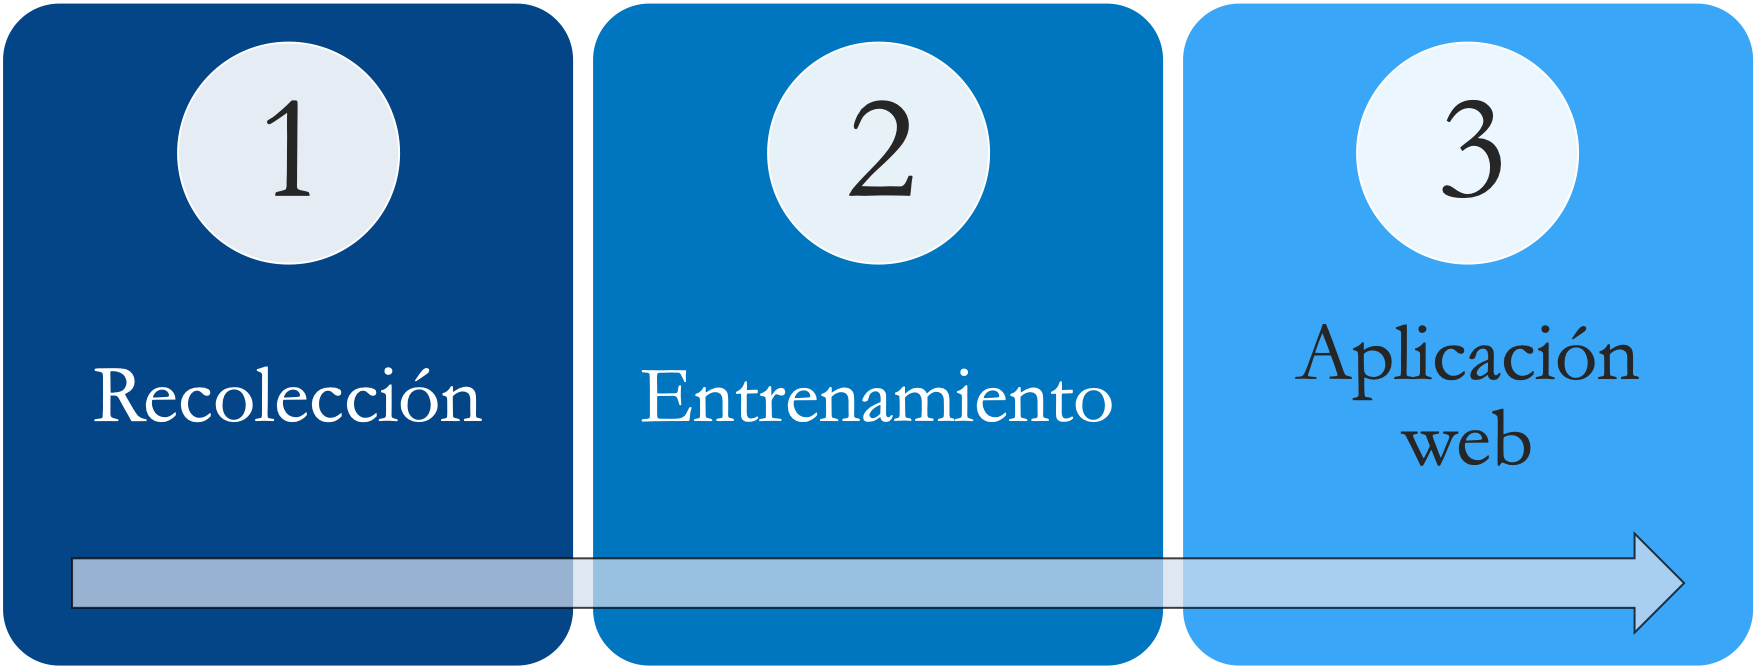
\includegraphics[scale=.35]{imagenes/Capitulo5/Etapas.png}
\caption{Etapas de desarrollo}
\label{fig:cp5:etapas}
\end{figure}
 

\section{Recolección}

%-------------------------------Recolección----------------------------------------------%

El proceso de recolección es parte fundamental del presente trabajo terminal, ya que permitió conformar el corpus necesario para llevar a cabo la etapa de entrenamiento, este proceso se llevo a cabo por etapas.

\begin{itemize}
	\item Seleccionar los sitios web
	\item Información a recolectar
	\item Análisis del sitio web
	\item Proceso de recolección
\end{itemize}

\subsection{Selección de sitios web}

Se han seleccionado los diarios Aristegui Noticias, El Economista, La Jornada, La Prensa, Proceso, Sopitas y TV Azteca para recolectar noticias, fueron seleccionados debido a que forman parte de los sitios web más consultados, sin embargo durante la etapa de recolección se descartaron ciertos sitios debido a que ya no permiten realizar \textit{web scraping}


\subsection{Información recolectada}

Se llevó a cabo un análisis acerca de la información que contiene cada una de las noticias y con base en ello se determinó recolectar la siguiente información:

\begin{itemize}
	\item URL de la noticia
	\item Título
	\item Fecha
	\item Sección
	\item Autor
	\item Descripción
	\item Noticia
\end{itemize}

Cabe destacar que no toda la información recuperada fue utilizada en el proceso de entrenamiento, sin embargo se considerarón los puntos anteriores ya que la mayor parte de las noticias cuentan con esa información.


\subsection{Análisis de sitios web}

Una vez definida la información requerida de cada noticia se realizó un análisis sobre la estructura HTML de cada sitio web, con el fin de realizar expresiones \textit{XPath} que nos permitieran recorrer y procesar un documento XML, dado que cada sitio web cuenta con una estructura diferente, fue necesario realizar el análisis de manera individual, cabe mencionar que existen sitios los cuales realizan actualizaciones a sus páginas por lo cual era necesario realizar el análisis cada dos meses.

Una expresión \textit{XPath} de ruta nos permite buscar y seleccionar los distintos nodos de un documento XML, en el siguiente Cuadro \ref{box:xmlEjemplo} se muestra un ejemplo de un documento XML.

\begin{mygraybox}[label={box:xmlEjemplo}]{Documento XML} 
<nota>\\
	<para>Daniel</para>\\
	<de>Andres</de>\\
	<titulo>Recordatorio</titulo>\\
	<texto>Don't forget me this weekend!</texto>\\
</nota>
\end{mygraybox}

\subsection{Proceso de recolección de noticias}

Existen diversas técnicas y herramientas para la recolección de información, sin embargo en el presente trabajo han sido utilizadas técnicas de \textit{web scraping}.

La siguiente Figura \ref{Fig:recoleccion} muestra el proceso que se lleva a cabo durante la recolección utilizando web scraping.

\begin{figure}[H]
	\centering
	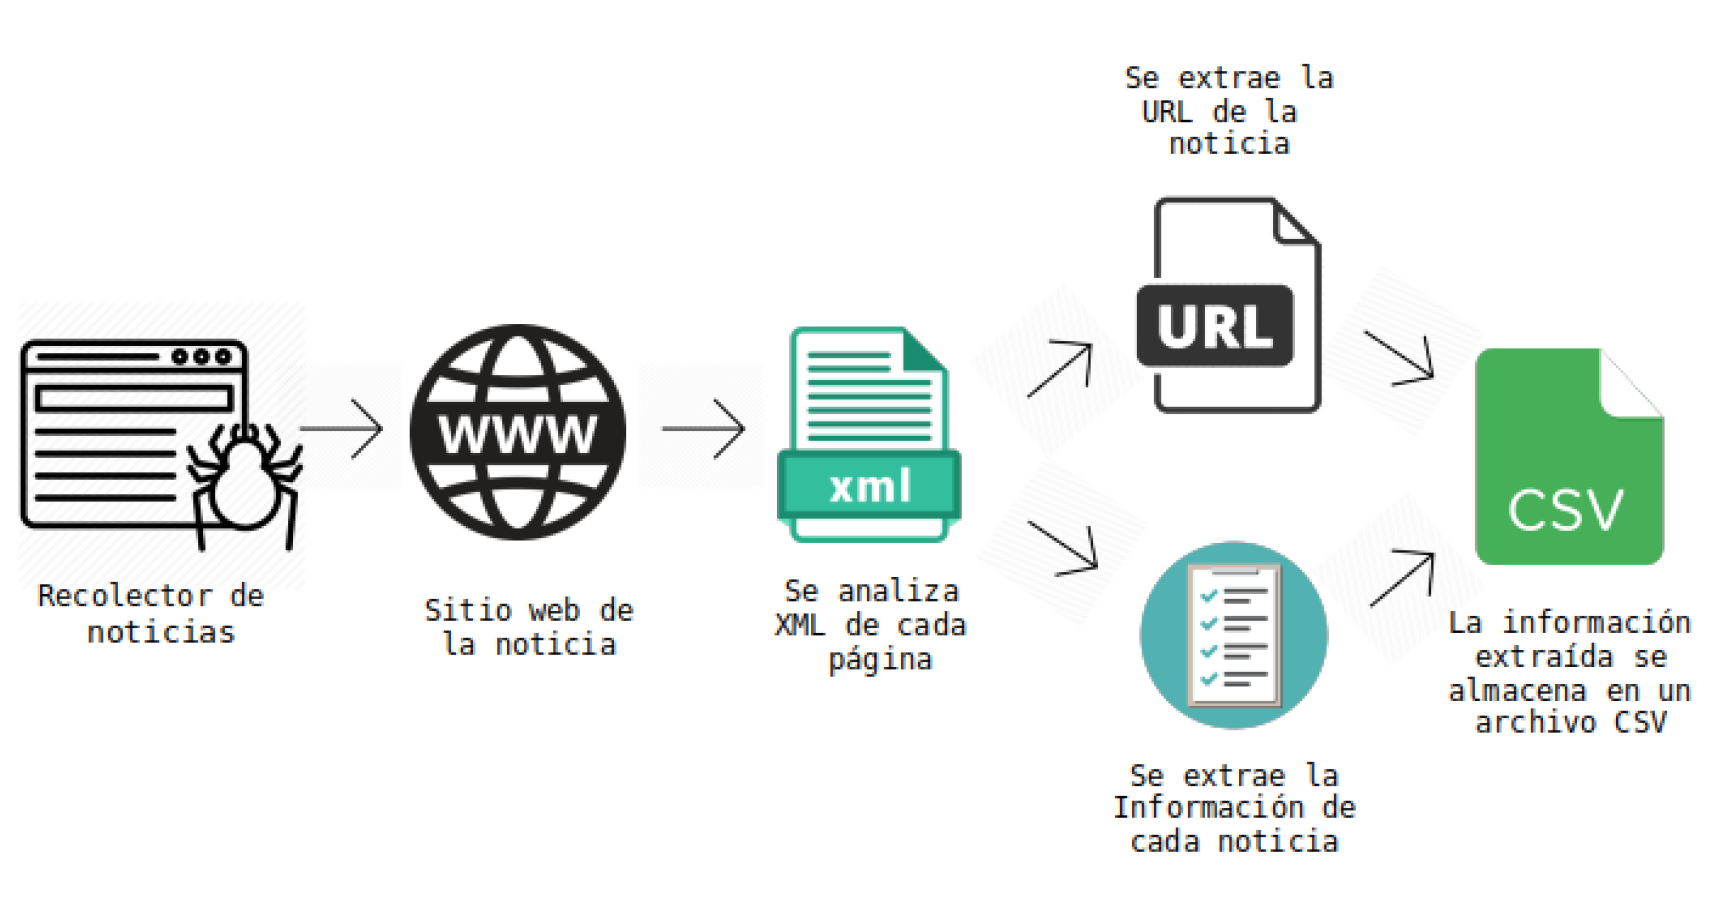
\includegraphics[scale=.2]{imagenes/Capitulo5/recoleccion.png}
	\caption{Proceso de recolección}
	\label{Fig:recoleccion}
\end{figure}

Es necesario contar con noticias de las secciones (Ciencia y Tecnología, Cultura, Deportes, Economía y Política), por lo cual se realizó un crawler por sección, con el fin enriquecer el número de noticias de cada sección, permitiendo obtener mejores resultados en la práctica.
\\
Para generar nuestro corpus, se recolectaron noticias durante el periodo de julio a septiembre con un intervalo de dos días, con el fin de no tener noticias repetidas y evitar ser bloqueados debido alnúmero de peticiones realizadas al sitio web. 
\\
Una vez finalizado el proceso de recolección los resultados obtenidos por sección se muestra en la Figura  \ref{Fig:notseccionV1}.

\begin{figure}[H]
	\centering
	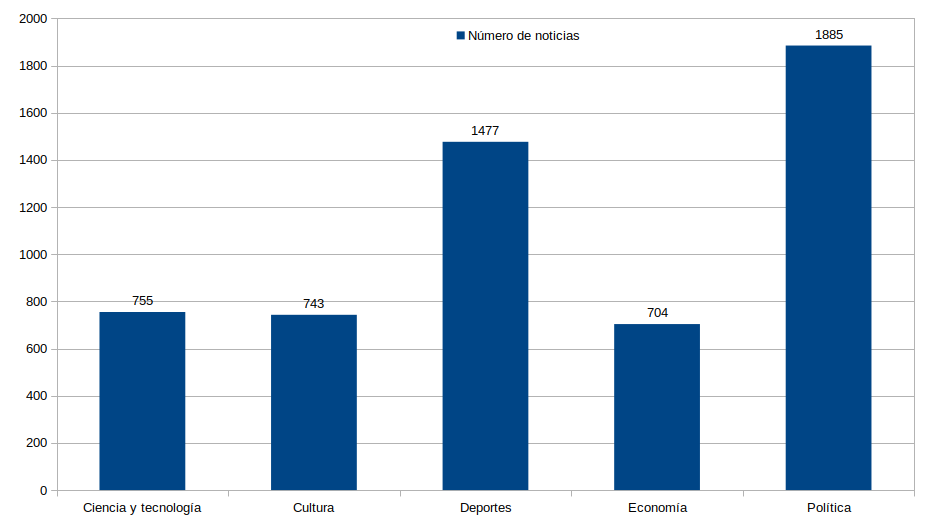
\includegraphics[scale=.6]{imagenes/Capitulo5/noticiasPorSeccionV1.png}
	\caption{Noticias recolectadas durante el primer corte.}
	\label{Fig:notseccionV1}
\end{figure}

Cabe destacar que el número de noticias por sección no se encontraba balanceado debido a que no existía un gran número de sitios que publicarán noticias de cultura, por ello se decidió continuar con el proceso de recolección de noticias, con el fin de balancear el corpus y así nuestros resultados obtenidos en la práctica fueran mejores.
\\
Una vez finalizada la segunda etapa de recolección los nuevos resultados se muestran en la Figura \ref{Fig:notseccion}

\begin{figure}[H]
	\centering
	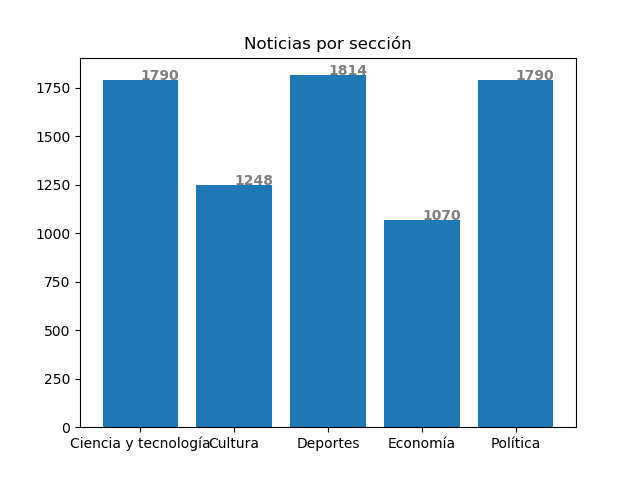
\includegraphics[scale=.6]{imagenes/Capitulo5/noticiasPorSeccion.png}
	\caption{Numero total de noticias recolectadas por sección.}
	\label{Fig:notseccion}
\end{figure}

Las resultados obtenidos por cada sitio web, se muestran en las siguientes Figuras.
\\
\begin{figure}[H]
	\centering
	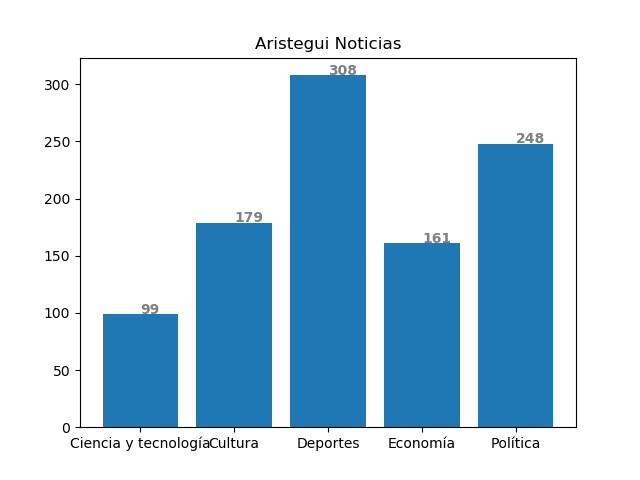
\includegraphics[scale=.45]{imagenes/Capitulo5/aristegui.png}
	\caption{Total de noticias recolectadas del sitio web de Aristegui Noticias}
	\label{Fig:notsitioaristegui}
\end{figure}

\begin{figure}[H]
	\centering
	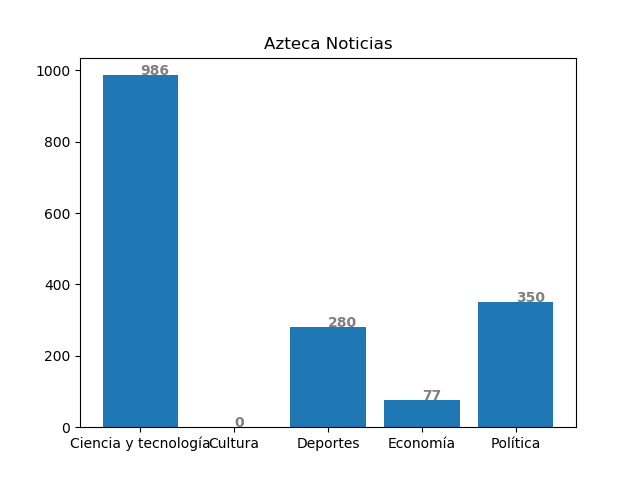
\includegraphics[scale=.45]{imagenes/Capitulo5/azteca.png}
	\caption{Total de noticias recolectadas del sitio web de Azteca Noticias}
	\label{Fig:notsitioazteca}
\end{figure}

\begin{figure}[H]
	\centering
	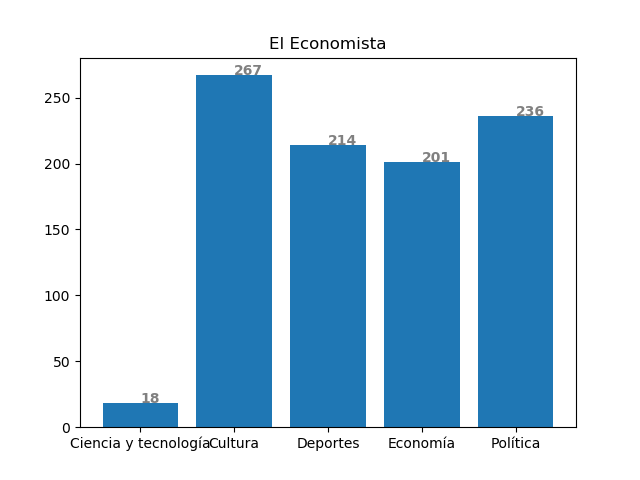
\includegraphics[scale=.45]{imagenes/Capitulo5/economista.png}
	\caption{Total de noticias recolectadas del sitio web de El Economista}
	\label{Fig:notsitioeconomista}
\end{figure}

\begin{figure}[H]
	\centering
	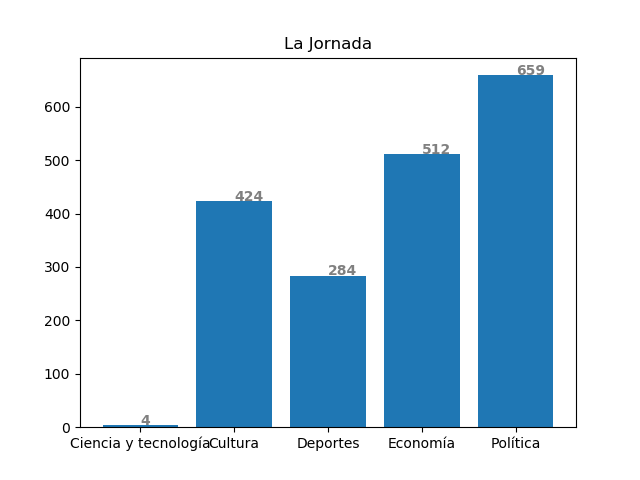
\includegraphics[scale=.45]{imagenes/Capitulo5/jornada.png}
	\caption{Total de noticias recolectadas del sitio web de La Jornada}
	\label{Fig:notsitiojornada}
\end{figure}

\begin{figure}[H]
	\centering
	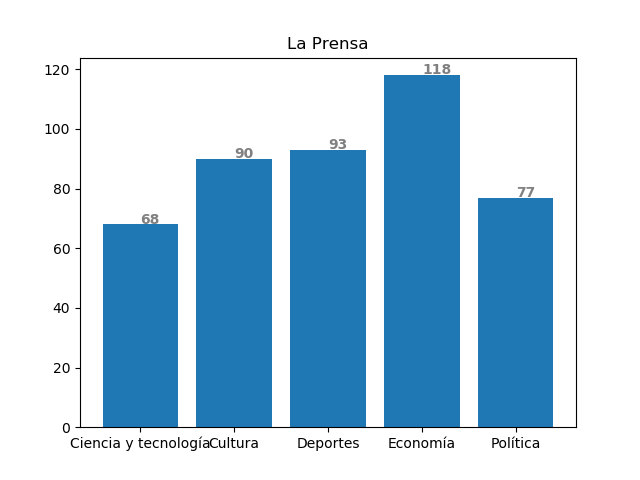
\includegraphics[scale=.45]{imagenes/Capitulo5/prensa.png}
	\caption{Total de noticias recolectadas del sitio web de La Prensa}
	\label{Fig:notsitioprensa}
\end{figure}

\begin{figure}[H]
	\centering
	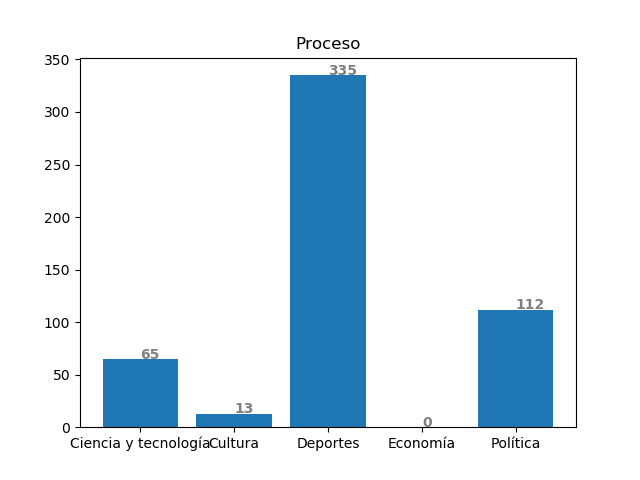
\includegraphics[scale=.45]{imagenes/Capitulo5/proceso.png}
	\caption{Total de noticias recolectadas del sitio web de Proceso}
	\label{Fig:notsitioproceso}
\end{figure}

\begin{figure}[H]
	\centering
	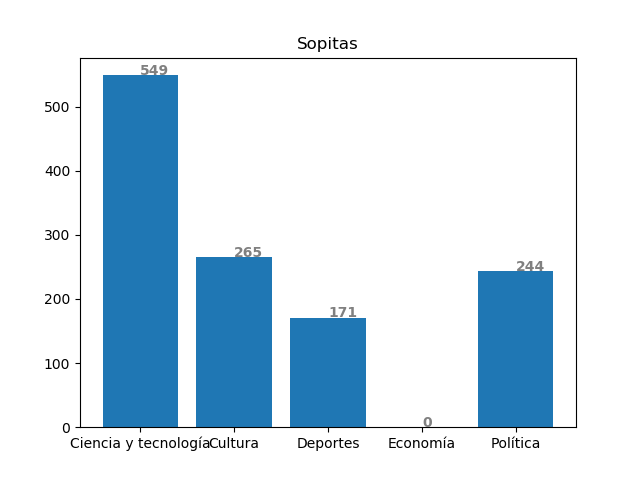
\includegraphics[scale=.45]{imagenes/Capitulo5/sopitas.png}
	\caption{Total de noticias recolectadas del sitio web de Sopitas}
	\label{Fig:notsitiosopitas}
\end{figure}

Una vez concluida la recolección de noticias se procedió con el balanceo de noticias quedando un total de 700 noticias por sección.
\newpage
\section{Entrenamiento de clasificador}
%\HSection{ENTRENAMIENTO}

El segundo pilar del trabajo terminal es entrenar un algoritmo (de aprendizaje automático), para clasificar las noticias en las secciones \textbf{Ciencia y tecnología}, \textbf{Política}, \textbf{Deportes}, \textbf{Economía} y \textbf{Cultura}. Cabe destacar que el clasificador resolverá un problema multiclase (ver \Tref{cp3:multinomial}{Clasificación multiclase}) debido a que la entrada es una artículo y como salida brinda la pertenencia a una sección  de 5 posibilidades. El proceso de entrenamiento se muestra en la Figura \ref{fig:cp5:procesoE}.\\



En este punto es importante mencionar que existe un trabajo terminal previo (TT 2017-A042) el cual ha generado un modelo para clasificar noticias por secciones, sin embargo existen diferencias importantes entre el TT 2017-A042 y el propuesto en este documento, las cuales son mostradas en la Figura \ref{cp5:diferenciastt}.



\begin{figure}[h]
\centering
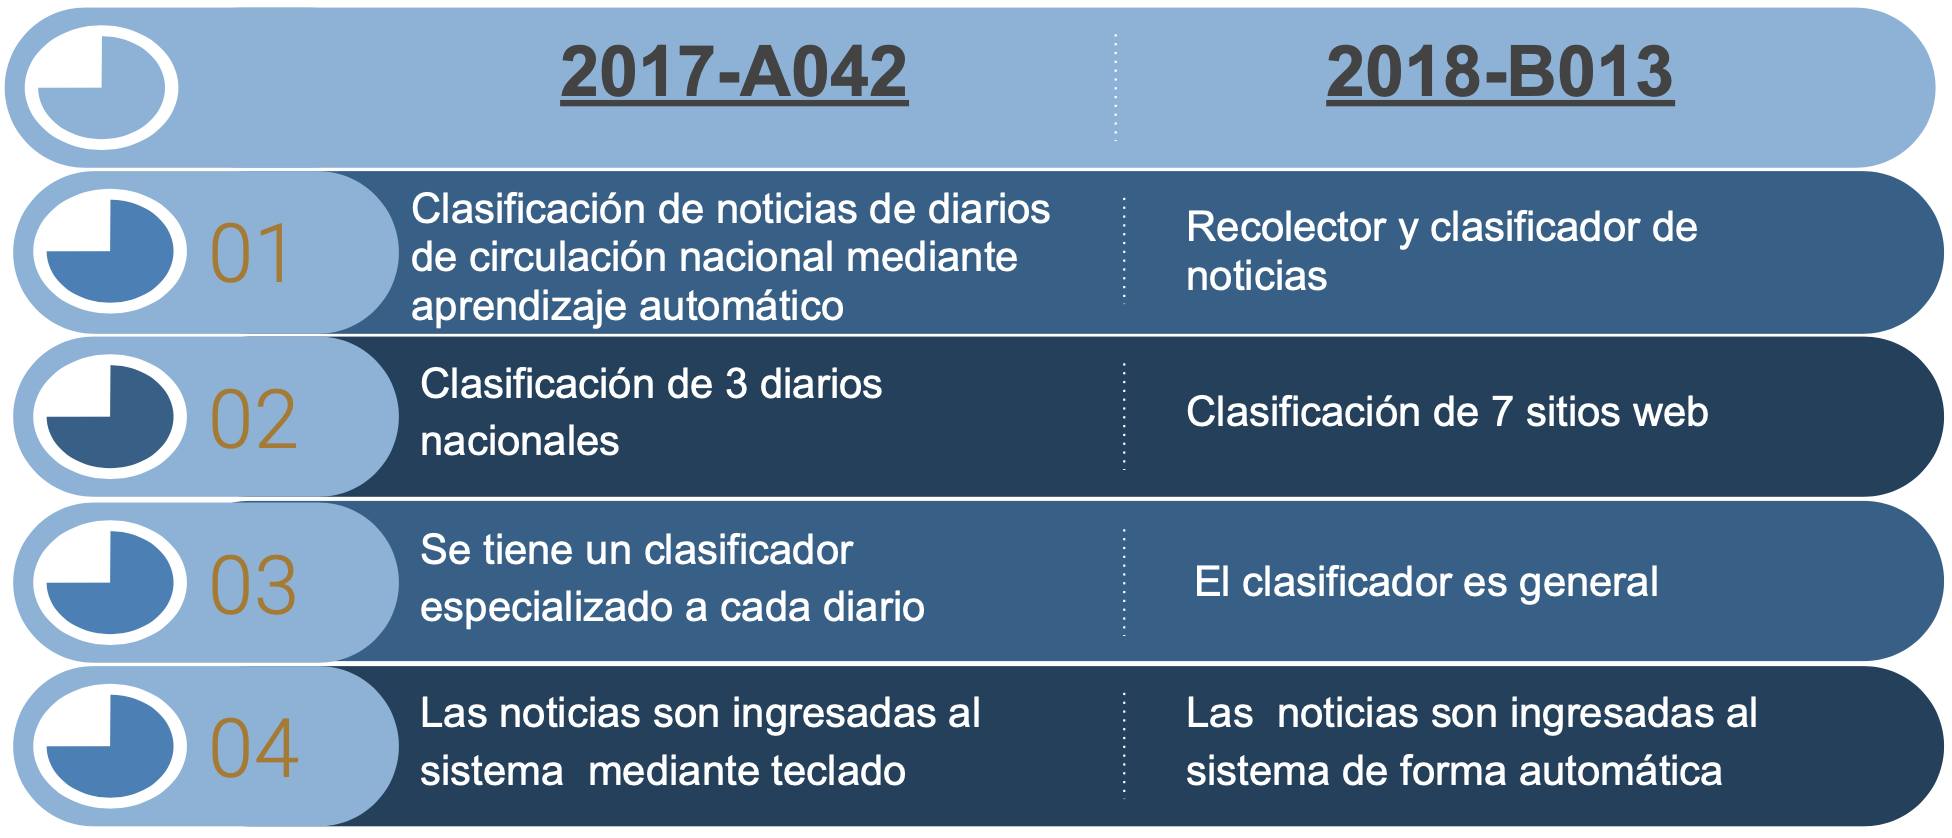
\includegraphics[scale=0.35]{imagenes/capitulo5/entrenamiento/diferenciastt.png}
\caption{Diferencias del clasificador en el TT 2017-A042 y 2018-B013}
\label{cp5:diferenciastt}
\end{figure} 

Como se puede observar en la Figura \ref{cp5:diferenciastt} el modelo del TT 2017-A042 está orientado en la clasificación de noticias de 3 diarios de circulación nacional (\textbf{El Universal}, \textbf{La Jornada} y \textbf{Excélsior}), además de estar enfocado en las secciones particulares de cada periódico y de haber entrenado un algoritmo por cada diario. Por otra parte, este trabajo terminal (TT 2018-B013) tiene como objetivo clasificar noticias en 5 secciones (\textbf{deportes}, \textbf{economía}, \textbf{política}, \textbf{cultura}, \textbf{ciencia y tecnología}), de 7 diferentes sitios web. Es importante mencionar que se entrenará un solo modelo el cual generalice la tarea de clasificación de todas las fuentes noticiosas.\\  

Dada las diferencias se decidió utilizar un nuevo corpus, así como entrenar un nuevo clasificador que se ajuste mejor al objetivo de este trabajo terminal.\\


Como se mencionó en la etapa de recolección, el corpus obtenido contiene 7,707 noticias en total. Sin embargo este contenido debe ser procesado y solo seleccionar los artículos que aporten información para el entrenamiento, al final de la etapa de pre\-procesamiento el corpus será dividió en dos conjuntos: entrenamiento con el 90\% de los artículos y prueba con el 10\%. A continuación se explica la etapa de \textbf{Pre-procesamiento}.\\

\begin{figure}[h]
\centering
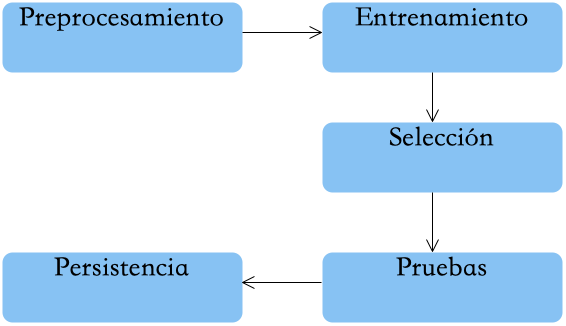
\includegraphics[scale=.55]{imagenes/capitulo5/Entrenamiento/Esquema.png}
\caption{Proceso de entrenamiento}
\label{fig:cp5:procesoE}
\end{figure}



%------------------------------------------------------------------%
\subsection{Preprocesamiento}

Como primera instancia, el corpus creado debe ser procesado, con el fin de crear vectores que representan el contenido de cada artículo de forma ordenada (ver \Tref{cp3:representaciont}{Representación del texto}), de esta manera los algoritmos de clasificación son capaces de entender la información. En cuanto a los datos que son procesados de la noticia cabe mencionar que solo se usa el título y la redacción del artículo, los demás datos (como url, fecha, sección) no son necesarios para el entrenamiento. Este proceso consta de 6 etapas, las cuales son mostradas en la Figura \ref{fig:cp5:preprocesamiento}. \\

Cabe destacar que estas etapas están desarrolladas en un script escrito en el lenguaje \textbf{python 3}, en cada sección se hará mención de las bibliotecas ocupadas.\\

\begin{figure}[h]
\centering
\includegraphics[scale=.55]{imagenes/capitulo5/Entrenamiento/preprocesamiento.png}
\caption{Etapas de preprocesamiento}
\label{fig:cp5:preprocesamiento}
\end{figure}

%----------------------------------%
%\begin{large}
\Tlabel{cp5:limpieza}
\subsubsection{Limpieza}
%\end{large}

Esta etapa consiste en eliminar texto que no brinda información útil para el entrenamiento como, hipertexto (ver \Tref{cp3:html}{HTML}), símbolos especiales (como \# $\dagger$ $\sqrt{ }$), \textit{emojis} (como \dSmiley \dCooley \dNinja). Por ejemplo el texto \ref{box:cp5:texto} muestra la redacción de una noticia con la información descargada de una pagina web. El resultado de limpiar la noticia se muestra en el texto \ref{box:cp5:limpio}. Se puede observar que se han eliminado los elementos $<p>\ </p>\ <!--\ -->$ \# $\dagger$ \dSmiley \dCooley \dInnocey.\\

Para realizar esta tarea se han utilizado las bibliotecas: \textbf{pandas} como medio de lectura de archivos tipo \textbf{CSV} (\textit{comma separeted values}, por sus siglas en ingles); \textbf{re} la cual permite evaluar expresiones regulares con el objetivo de eliminar símbolos; \textbf{demoji} quien permite eliminar \textit{emojis} dentro del texto.\\

\begin{mygraybox}[label={box:cp5:texto}]{Texto de entrada} 
$<p>\dagger$$\ \ \ $ El número 343 de El Trimestre Económico,$\otimes$ revista emblemática del Fondo de Cultura 
$<!--\ -->$
Económica (FCE), será * * * presentado por David Ibarra Muñoz \dSmiley , Carlos Tello Macías \dCooley , Alicia Puyana \dInnocey y Pablo Ruiz Nápoles el martes 27 de agosto a las 6 de la tarde, en la librería Rosario Castellanos, ubicada en avenida Tamaulipas \# 202, en la colonia Condesa de la capital mexicana.$</p>$
\end{mygraybox}

\ \\

\begin{mygraybox}[label={box:cp5:limpio}]{Texto limpio} 
El número 343 de El Trimestre Económico, revista emblemática del Fondo de Cultura 
Económica (FCE), será presentado por David Ibarra Muñoz, Carlos Tello Macías , Alicia Puyana y Pablo Ruiz Nápoles el martes 27 de agosto a las 6 de la tarde, en la librería Rosario Castellanos, ubicada en avenida Tamaulipas 202, en la colonia Condesa de la capital mexicana.
\end{mygraybox}
%----------------------------------%
%\begin{large}
\subsubsection{Filtro de longitud}
%\end{large}

Con base en la regla de negocio \RNref{RN1}{Número de palabras} se ha definido 180 palabras como longitud mínima de las noticias, incluyendo en la definición de palabra números, signos de puntuación y exclamación.
Para esto después de haber concluido el proceso de limpieza se pregunta por la longitud de la cadena (sin contar los espacios) y si esta es mayor o igual a 180, entonces es un artículo válido para utilizar en el entrenamiento de lo contrario no es tomado en cuenta.\\


%----------------------------------%
%\begin{large}
\subsubsection{Delimitación del corpus}
%\end{large}

En este punto del proceso, la cantidad de artículos ha disminuido (como se observa en la Figura \ref{fig:cp5:noticiasSecciones}), sin embargo la distribución por sección no es homogénea, esta situación crea un sesgo en el corpus y después en la etapa de \textbf{Entrenamiento} los algoritmos pueden desarrollar una preferencia por la categoría con mas datos. Por está razón se debe acotar la cantidad de noticias.\\

Como se muestra en la Figura \ref{fig:cp5:noticiasSecciones} cada sección contiene al menos 700 noticias, por lo tanto este es el número definido para delimitar el número de artículos. De esta manera el corpus se ha definido como se muestra en la Figura \ref{fig:notBalanceadas}, obteniendo un total de 3,500 noticias.\\

\begin{figure}[H]
	\centering
	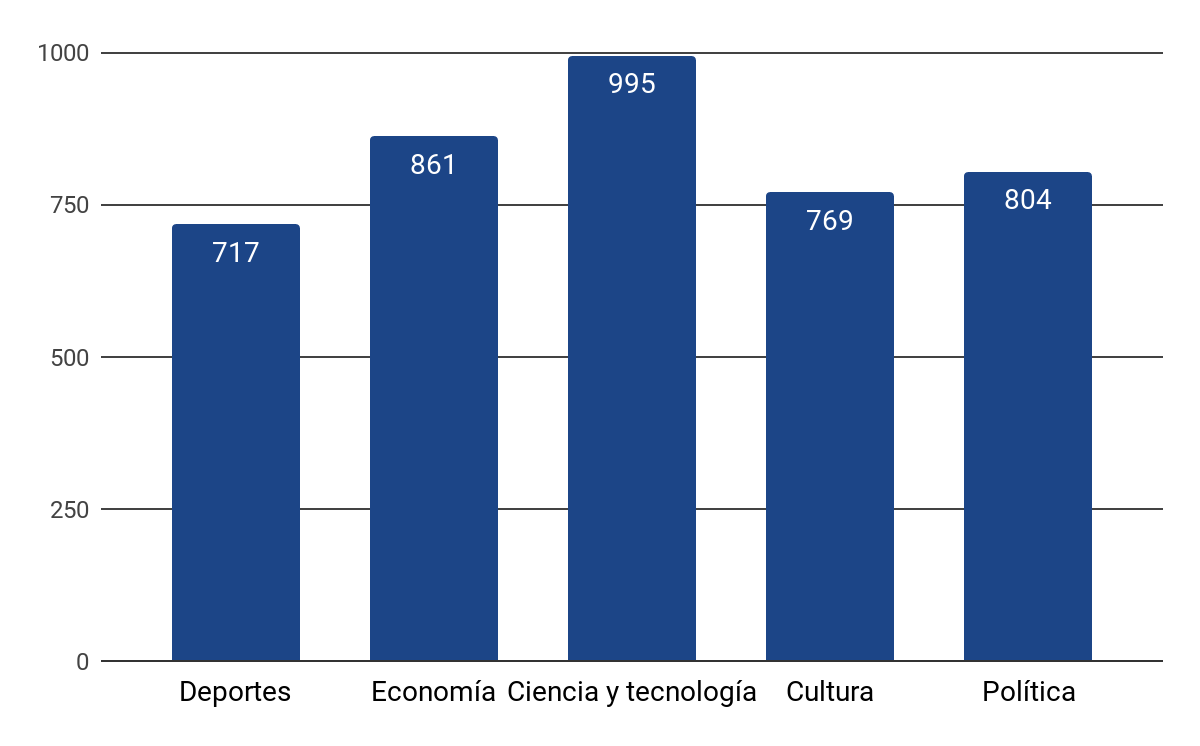
\includegraphics[scale=.33]{imagenes/Capitulo5/Entrenamiento/noticiasSecciones.png}
	\caption{Noticias por sección}
	\label{fig:cp5:noticiasSecciones}
\end{figure}


\begin{figure}[H]
	\centering
	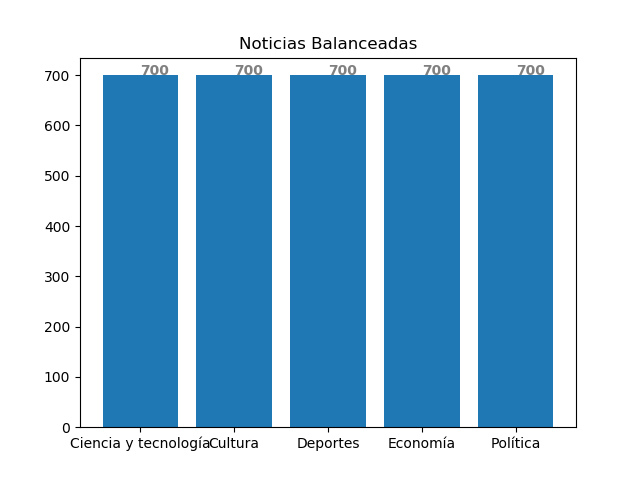
\includegraphics[scale=.5]{imagenes/Capitulo5/noticiasBalanceadas.png}
	\caption{Noticias por sección}
	\label{fig:notBalanceadas}
\end{figure}

%----------------------------------%
%\begin{large}
\subsubsection{Tokenizar}
%\end{large}
\Tlabel{cp5:tokenizacion}
La etapa de tokenización consiste en separar el texto en sus elementos mínimos llamados tokens, donde se separan palabras, signos de puntuación, llaves y números mediante un espacio. Continuando con el ejemplo \ref{box:cp5:limpio} donde el texto se encuentra limpio, se procede a su tokenización. El resultado es mostrado en el Cuadro \ref{box:cp5:tokenizar}. Para remarcar el ejemplo observe la palabra entre paréntesis \textbf{(FCE)} la cual es separada en \textbf{( FCE )} mostrando que ahora cada elemento representa un token individual. Para el desarrollo de esta tarea se utilizó la biblioteca \textbf{RegexpTokenizer}.\\

\begin{mygraybox}[label={box:cp5:tokenizar}]{Texto tokenizado} 
El número 343 de El Trimestre Económico , revista emblemática del Fondo de Cultura 
Económica ( FCE ) , será presentado por David Ibarra Muñoz , Carlos Tello Macías , Alicia Puyana y Pablo Ruiz Nápoles el martes 27 de agosto a las 6 de la tarde , en la librería Rosario Castellanos , ubicada en avenida Tamaulipas 202 , en la colonia Condesa de la capital mexicana .
\end{mygraybox}

%----------------------------------%
%\begin{large}
\subsubsection{Lematizar}
%\end{large}
\Tlabel{cp5:lematizacion}
Lematizar es el proceso de reducir cada palabra a su lema, con el fin de disminuir la dispersión en el texto, por ejemplo las palabras correrás, corriendo, corrí, tienen como lema el verbo correr, el plural niños tiene como lema niño (ver \Tref{cp3:lematizacion}{Lematización}). Para realizar esta tarea se ha usado \textbf{spacy} el cual es una librería de código abierto, con el diccionario \textit{es\_core\_news\_sm} quien permite analizar el léxico del lenguaje español.\\

Siguiendo con las etapas del proceso se toma el texto \ref{box:cp5:tokenizar} como entrada al programa y este da como salida el texto que se muestra en el Cuadro \ref{box:cp5:lematizado}.\\

\begin{mygraybox}[label={box:cp5:lematizado}]{Texto lematizado} 
el número 343 de el trimestre económico , revista emblemático del fondo de cultura económica ( fce ) , ser presentar por david ibarra muñoz , carlos tello macías , alicia puyana y pablo ruiz nápoles el martes 27 de agostar a los 6 de lo tardar , en lo librería rosario castellanos , ubicar en avenir tamaulipas 202 , en lo colonia condesa de lo capital mexicano .
\end{mygraybox}
\ \\

Cuando el proceso de lematización concluye se genera un identificador único para cada noticia el cual se define de la siguiente forma 

\begin{equation*}
id=<Identificador\ de\ sitio\ web><Numero\ de\ noticias>
\end{equation*}
 
donde \textbf{Identificador de sitio web} define un número único para hacer referencia a los sitios web (ver Tabla \ref{tab:cp5:sitioweb}) y  \textbf{Número de noticias} es el número del artículo.

\begin{table}[h]
\centering
	\begin{tabular}{|l|l|}
	%-----------------------Ecanbezado-----------------------------------%
		\hline
		\multicolumn{1}{| >{\columncolor{white!30!black}}l|}{ \textcolor{myWhite}{\textbf{Número}} }&
		\multicolumn{1}{| >{\columncolor{white!30!black}}l|}{ \textcolor{myWhite}{\textbf{Página web}} }\\
		\hline
	%------------------------------------------------%

		\textbf{100} & Aristegui noticias\\
		\hline
		\textbf{200} & Tv azteca\\
		\hline

		\textbf{300} & El economista\\
		\hline

		\textbf{400} & La jornada\\	
		\hline

		\textbf{500} & La prensa\\
		\hline

		\textbf{600} & Proceso\\
		\hline

		\textbf{700} & Sopitas\\
		\hline

	\end{tabular}\\
\caption{Identificador de sito web}
\label{tab:cp5:sitioweb}
\end{table}


Como segundo paso las noticias son almacenadas en un archivo con extensión \textbf{TXT}, los elementos por almacenar son \textbf{id}, \textbf{titulo}, \textbf{noticia} y \textbf{sección}, los cuales son separados por los caracteres \&\&\&\&\&. El Cuadro \ref{box:cp5:archivo} muestra un ejemplo de la estructura del archivo.\\

\begin{mygraybox}[label={box:cp5:archivo}]{Estructura de archivo} 
\textbf{id}\&\&\&\&\&\textbf{titulo}\&\&\&\&\&\textbf{noticia}\&\&\&\&\&\textbf{seccion}\\
1001\&\&\&\&\&Titulo 1\&\&\&\&\&Contenido noticia 1\&\&\&\&\&0\\
...\\
5003500\&\&\&\&\&Titulo 3500\&\&\&\&\&Contenido noticia 3500\&\&\&\&\&4
\end{mygraybox}

%----------------------------------%

%\begin{large}
\Tlabel{cp5:divisionC}
\subsubsection{División del corpus}
%\end{large}


Para el correcto diseño y evaluación del algoritmo clasificador se requiere dividir el corpus en dos conjuntos: \textbf{entrenamiento} y \textbf{prueba}, con un 90\% y 10\% del total del corpus respectivamente. En cada grupo deben estar repartidas noticias de las 5 secciones definidas, sin embargo los artículos almacenados están ordenados de forma descendente como: \textbf{Deportes}, \textbf{Economía}, \textbf{Política}, \textbf{Cultura}, \textbf{Ciencia y tecnología}, para seleccionar de forma distribuida los datos se ha utilizado una técnica llamada \textit{Shuffle}.\\

\textit{Shuffle} consiste en brindar un arreglo con los identificadores de las noticias y un número (nombrado usualmente como semilla), quien generar un nuevo orden en los identificadores de acuerdo a los números pseudo aleatorios que retorna esta función, tomando este como el nueva orden de los textos en el archivo de almacenamiento. Para el desarrollo de esta etapa se ha utilizado la biblioteca \textbf{Shuffle} con una semilla de 5.\\

Para ilustrar un ejemplo, en el cuadro \ref{box:cp5:ids} se muestra un conjunto de identificadores ordenados por el último número del $id$, al utilizar la función \textit{Shuffle} con una semilla de 2, se genera un nuevo orden el cual es mostrado en el Cuadro \ref{box:cp5:shuffle}.\\


\begin{mygraybox}[label={box:cp5:ids}]{Identificadores de noticias} 
\begin{equation*}
\begin{bmatrix}
1001 & 2002 & 3003 & 4004 & 5005 & 6006 & 7007 & 1008\\ 
\end{bmatrix}
\end{equation*}
\end{mygraybox}


\begin{mygraybox}[label={box:cp5:shuffle}]{Nuevo orden de ID's} 
\begin{equation*}
\begin{bmatrix}
5005 & 2002 & 7007 & 3003 & 4004 & 1008 & 6006 & 1001\\
\end{bmatrix}
\end{equation*}
\end{mygraybox}

La distribución generada por esta función es almacenada en un archivo, y como último paso se han tomado las primeras 350 noticias de forma manual y se han colocado en un archivo diferente, definido así las noticias de entrenamiento (con 3,150) y de prueba (con 350).\\

La cantidad de noticias por sección del conjunto de entrenamiento se muestran en la Figura \ref{fig:cp5:seccionE} y del conjunto de prueba en la Figura \ref{fig:cp5:seccionP}.



\begin{figure}[H]
\centering
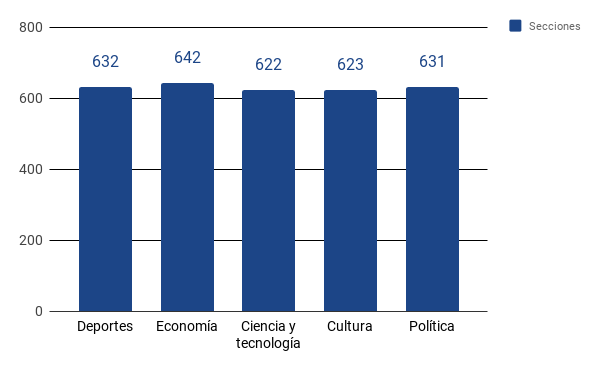
\includegraphics[scale=.67]{imagenes/capitulo5/Entrenamiento/SeccionesE.png}
\caption{Corpus de entrenamiento}
\label{fig:cp5:seccionE}
\end{figure}

\begin{figure}[H]
\centering
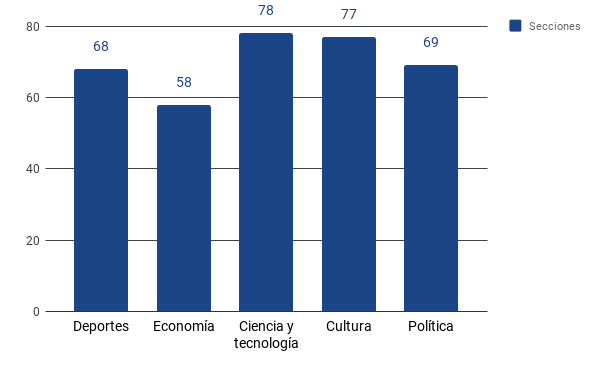
\includegraphics[scale=.67]{imagenes/capitulo5/Entrenamiento/SeccionesP.png}
\caption{Corpus de prueba}
\label{fig:cp5:seccionP}
\end{figure}

%\begin{figure}[h]
%\centering
%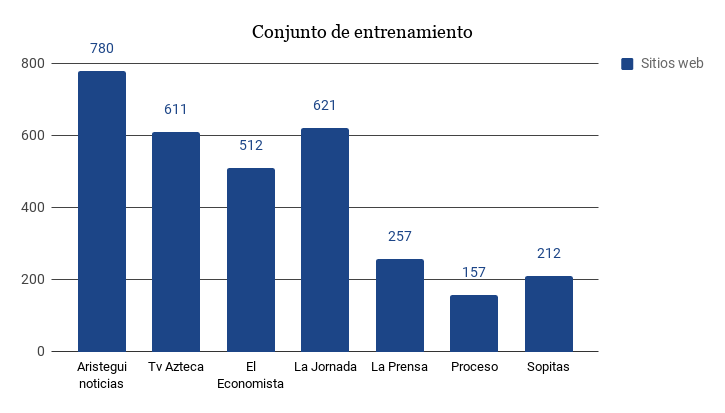
\includegraphics[scale=.6]{imagenes/capitulo5/Entrenamiento/SitiosE.png}
%\caption{Número de noticias pertenecientes a los sitios web}
%\label{fig:cp5:sitiosE}
%\end{figure}



%------------------------------------------------------------------%
\subsection{Entrenamiento}

Para crear un modelo clasificador usando aprendizaje supervisado (ver \Tref{cp3:asupervisado}{Aprendizaje supervisado}), se debe construir dos conjuntos etiquetados: entrenamiento para el proceso de aprendizaje y otro de prueba, para medir su precisión. En la sección anterior estos grupos se han formado con noticias de 5 secciones: \textbf{Deportes}, \textbf{Economía}, \textbf{Política}, \textbf{Cultura}, \textbf{Ciencia y tecnología}. Ambos conjuntos de datos serán usados por 4 algoritmos (seleccionados con base en el estado del arte ver \Tref{cp2:estadodelarte}{Estado del arte}), los cuales son:

\begin{itemize}
	\item \textbf{Naive Bayes} (ver \Tref{cp3:naive}{Naive Bayes})
	\item \textbf{Regresión logística} (ver \Tref{cp3:regresion}{Regresión logística})
	\item \textbf{Máquina de soporte vectorial} (ver \Tref{cp3:msv}{MSV})
	\item \textbf{Random Forest} (ver \Tref{cp3:random}{Random Forest})
\end{itemize}

El proceso de entrenamiento consta de 5 pasos los cuales se muestran en la Figura \ref{fig:cp5:entrenamiento}.

\begin{figure}[h]
\centering
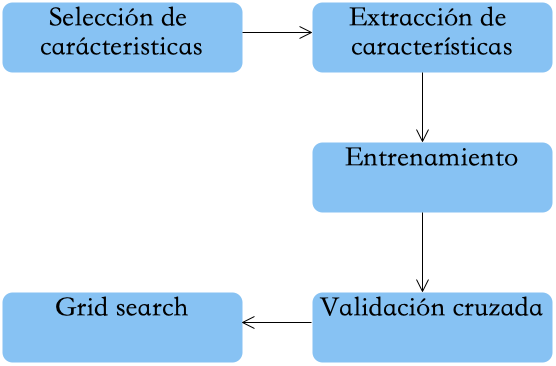
\includegraphics[scale=.55]{imagenes/capitulo5/Entrenamiento/Entrenamiento.png}
\caption{Etapas de entrenamiento}
\label{fig:cp5:entrenamiento}
\end{figure}

El desarrollo se ha implementado en el lenguaje de programación \textbf{Python 3}, utilizando la biblioteca \textbf{scikit learn} quien permite crear instancias de los algoritmos mencionados.\\

Como primer paso del entrenamiento, el corpus debe ser representado mediante conjuntos de vectores numéricos, esta es llamada representación vectorial (ver \Tref{cp3:representaciont}{Representación del texto}). Para lograr este objetivo, del corpus se deben seleccionar características que definan los elementos del vector numérico.\\

%----------------------------------%
%\begin{large}
\Tlabel{cp5:extraccion}
\subsubsection{Extracción de características}
%\end{large}

La extracción de características cuenta con dos tareas importantes: extraer el vocabulario y crear un vector de características.\\

Cada clase de noticias contiene un conjunto de palabras que son comunes en su ámbito, al analizar el léxico usado se observa los tecnicismos usados, por ejemplo en la sección deportes se ocupa, fútbol, jugador, ganador; en política, presidente, corrupción, PRI; en ciencia y tecnología, investigación, descubrimiento, publicación y así sucesivamente, por lo tanto estos vocablos pueden ser definidos como características que identifican a una sección. En este sentido la extracción de características es el proceso de tomar las palabras de las noticias para formar un vocabulario.\\

Para ejemplificar esta tarea observe el Cuadro \ref{box:cp5:corpus} el cual es un corpus de 4 oraciones. Una vez realizado el proceso de extracción de características se obtiene el vocabulario el cual el mostrado en el Cuadro \ref{box:cp5:caracteristicas}.\\

\begin{mygraybox}[label={box:cp5:corpus}]{Corpus} 
\begin{equation*}
\begin{bmatrix}
Este&es&la&primera&noticia&noticia\\
Esta&noticia&es&la&segunda&noticia&???\\
Y&este&es&la&tercera\\
Es&este&la&primera&noticia&????\\
\end{bmatrix}
\end{equation*}
\end{mygraybox}
\ \\
\begin{mygraybox}[label={box:cp5:caracteristicas}]{Selección de características} 
\begin{equation*}
\begin{bmatrix}
es & esta & este & la & noticia & primera & segunda & tercera & y & ?
\end{bmatrix}
\end{equation*}
\end{mygraybox}

%----------------------------------%



Después de extraer el  vocabulario, se crea un espacio vectorial por cada noticia donde cada elemento del vector representa la presencia o ausencia de una característica (palabra). Cabe mencionar que las características son extraídas de 2 formas, binario (donde 1 representa la presencia de la característica y 0 la ausencia ) y por frecuencia (donde se cuenta el número de veces que cada característica aparece). Continuando con el ejemplo del Cuadro \ref{box:cp5:corpus} se extraen las características por frecuencia y el resultado se muestra en el Cuadro \ref{box:cp5:frecuencia}, mientras que el Cuadro \ref{box:cp5:binario} muestra las características extraídas de forma binaria.\\

Para el desarrollo de esta etapa se ha utilizado la biblioteca \textbf{CountVectorizer} quien permite generar la selección y extracción de características, ademas esta es la representación vectorial (de cada noticia) que los algoritmos de clasificación pueden entender y por ende ser entrenados. Cabe destacar que la representación vectorial usada en este trabajo ha sido de forma binaria.\\

\begin{mygraybox}[label={box:cp5:frecuencia}]{Representación por frecuencia} 
\begin{equation*}
\begin{bmatrix}
1 & 0 & 1 & 1 & 2 & 1 & 0 & 0 & 0 & 0\\
1 & 1 & 0 & 1 & 2 & 0 & 1 & 0 & 0 & 3\\
1 & 0 & 1 & 1 & 1 & 0 & 0 & 1 & 1 & 0\\
1 & 0 & 1 & 1 & 1 & 1 & 0 & 0 & 0 & 4\\
\end{bmatrix}
\end{equation*}
\end{mygraybox}

\ \\

\begin{mygraybox}[label={box:cp5:binario}]{Representación binaría} 
\begin{equation*}
\begin{bmatrix}
1 & 0 & 1 & 1 & 1 & 1 & 0 & 0 & 0 & 0\\
1 & 1 & 0 & 1 & 1 & 0 & 1 & 0 & 0 & 1\\
1 & 0 & 1 & 1 & 1 & 0 & 0 & 1 & 1 & 0\\
1 & 0 & 1 & 1 & 1 & 1 & 0 & 0 & 0 & 1\\
\end{bmatrix}
\end{equation*}
\end{mygraybox}

\ \\
%----------------------------------%

%\begin{large}
\subsubsection{Entrenamiento}
%\end{large}


El corpus contiene noticias de varias fuentes, en  las cuales la redacción, coherencia, semántica varía, incluso en la edición de una misma noticia, por lo tanto en el entrenamiento se busca generalizar la clasificación de los artículos, analizando el texto como un conjunto de palabras, sin tomar en cuenta la semántica, esta técnica es llamada bolsa de palabras (ver \Tref{cp3:bolsap}{Bolsa de palabras}).\\

En este punto del trabajo las noticias están representadas en un espacio vectorial, y serán usadas en el proceso de entrenamiento de los algoritmos: \textbf{Naive Bayes}, \textbf{Regresión logística}, \textbf{Máquina de soporte vectorial}, \textbf{Random Forest}. Cada clasificador recibe como entrada un conjunto de vectores etiquetados y como salida se genera un modelo el cual predice la sección de nuevas noticias.\\ 

Para este trabajo se han definido las etiquetas como se muestra en la Tabla \ref{tab:cp5:etiquetas}, esta correspondencia es de secciones de noticias a un número único.\\


\begin{table}[h]
\centering
	\begin{tabular}{|l|l|}
	%-----------------------Ecanbezado-----------------------------------%
		\hline
		\multicolumn{1}{| >{\columncolor{white!30!black}}l|}{ \textcolor{myWhite}{\textbf{Sección}} }&
		\multicolumn{1}{| >{\columncolor{white!30!black}}l|}{ \textcolor{myWhite}{\textbf{Etiqueta}} }\\
		\hline
	%------------------------------------------------%

		\textbf{Deportes} & 0 \\
		\hline

		\textbf{Economía} & 1 \\
		\hline
		\textbf{Política} & 2 \\
		\hline

		\textbf{Cultura} & 3 \\
		\hline

		\textbf{Ciencia y tecnología} & 4 \\	
		\hline

	\end{tabular}\\
\caption{Etiquetas de secciones}
\label{tab:cp5:etiquetas}
\end{table}


El desarrollo ha utilizado una instancia de cada algoritmo, para esto se incluye la biblioteca correspondiente de \textbf{sciktlearn}, las cuales se muestran en la Tabla \ref{tab:cp5:librerias}, la entrada al clasificador es el conjunto de características y las etiquetas correspondientes, esto regresa como resultado un modelo que es capaz de predecir la sección de noticias, sin que estas estén etiquetadas.

\begin{table}[h]
\centering
	\begin{tabular}{|l|l|}
	%-----------------------Ecanbezado-----------------------------------%
		\hline
		\multicolumn{1}{| >{\columncolor{white!30!black}}l|}{ \textcolor{myWhite}{\textbf{Sección}} }&
		\multicolumn{1}{| >{\columncolor{white!30!black}}l|}{ \textcolor{myWhite}{\textbf{Etiqueta}} }\\
		\hline
	%------------------------------------------------%

		\textbf{Naive Bayes} & MultinomialNB \\
		\hline

		\textbf{Máquina de soporte vectorial} & SVC\\
		\hline

		\textbf{Regresión logísitica} &LogisticRegression\\
		\hline

		\textbf{Random Forest} &  RandomForestClassifier\\
		\hline

	\end{tabular}\\
\caption{Biblioteca de algoritmo}
\label{tab:cp5:librerias}
\end{table}




%----------------------------------%

%\begin{large}
\subsubsection{Validación cruzada}
%\end{large}

En el proceso de entrenamiento, los clasificadores reciben un conjunto noticias para ser entrenados y otro para realizar pruebas, sin embargo la selección de los artículos puede ser manipulada para obtener un resultado a conveniencia, siendo esto una mala práctica, por esta razón y en con el objetivo de obtener resultados mas robustos se ha implementado un técnica llamada Validación cruzada (ver \Tref{cp3:validacionc}{Validación cruzada}).\\

Este método consiste en tres pasos: el primero es dividir el corpus en entrenamiento y prueba (este conjunto es llamado pliegue); después se calcula la exactitud de la prueba y es almacenado; como último etapa los dos primeros paso son repetidos $n$ veces y para terminar  se calcula el promedio de la exactitud. En términos generales este promedio nos brinda mayor confianza en el resultado del entrenamiento de cada clasificador.\\

%----------------------------------%

%\begin{large}
\subsubsection{Ajuste de parámetros}
%\end{large}

Como se ha visto, los resultados de la clasificación son medidos por la cantidad de noticias correctas clasificadas, no obstante estos resultados pueden incrementar o decrementar con base a los parámetros ingresados a cada algoritmo.\\

Esta etapa consiste en observar el mejor resultado en la clasificación con los diferentes algoritmos, variando los parámetros y aplicar validación cruzada para medir la precisión. Para ejemplificar este tarea la Figura \ref{fig:cp5:gridbayes} muestra la variación del parámetro \textbf{alpha} en el algoritmo \textbf{Naive bayes} (este parámetro será explicado mas adelante) tomando los valores: 0.5, 1.0, 1.5 y 2.0, aplicando 2 pliegues en la validación cruzada.\\

\begin{figure}[h]
\centering
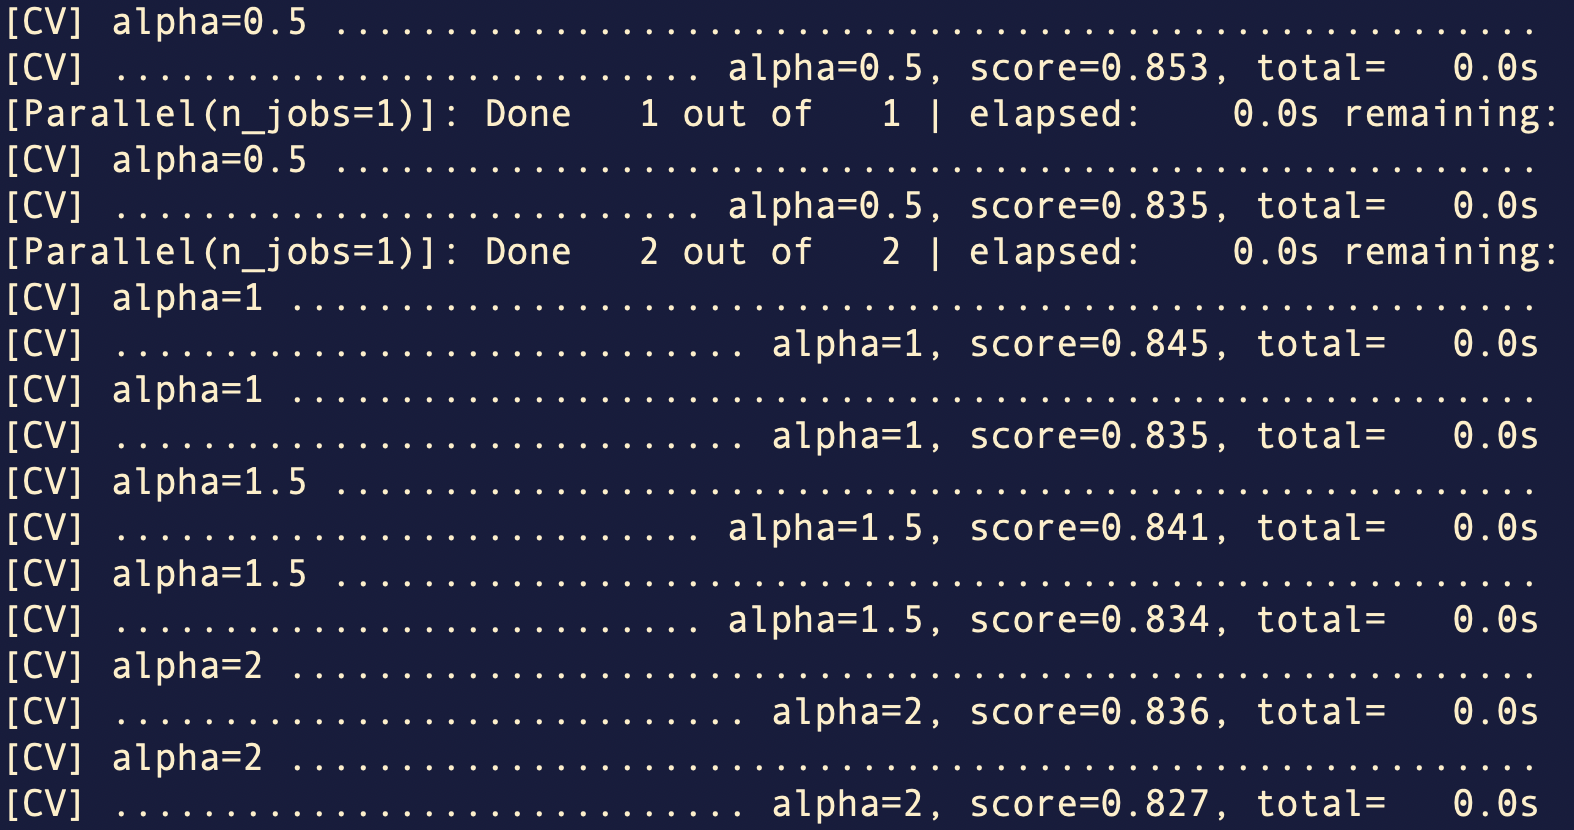
\includegraphics[scale=.5]{imagenes/capitulo5/Entrenamiento/gridbayes.png}
\caption{Corpus de entrenamiento}
\label{fig:cp5:gridbayes}
\end{figure}

Se observa que por cada parámetro implementado en la validación cruzada se muestra el resultado \textbf{score}, el cual es el promedio de la precisión de dicha prueba, se puede observar que el mejor resultado ha sido hecha con el $\alpha=0.5$, con un 85\% de precisión.\\


A continuación se explican los parámetros de cada clasificador: \\

%----------------%
%\begin{Text}
\textbf{Naive Bayes}\\
%\end{Text}
 
El parámetro en el cual se varía en este algoritmo, es un escalar llamado \textbf{Alpha} ($\alpha$). Este es un valor numérico asignado a cada palabra en el corpus con respecto a la frecuencia de aparición en un clase. El valor $\alpha$ evita que la importancia de una palabra se haga cero, \textbf{Alpha} es variado en los valores [$0.5, 1.0, 1.5, 2$].\\


%----------------%
%\begin{Text}
\textbf{Regresión logística}\\
%\end{Text}

%Referencia: https://www.kaggle.com/joparga3/2-tuning-parameters-for-logistic-regression
 Este algoritmo está basado en una regresión lineal y el calculo de probabilidades como se explica en el capitulo 3 (ver \Tref{cp3:regresion}{Regresión logística}). Existen 2  parámetros importantes en este clasificador, optimizando la función $l_1$  y minimizando el costo de la función $l_2$, en el cual existe un escalar $C$, donde: para valores pequeños de este número, los valores de los pesos $w$ (la importancia de cada palabra) se decrementa, teniendo así un modelo muy simple (se pierde información), de lo contrario para valores grandes de $C$ la complejidad del modelo aumenta pero se incrementa el ruido.\\

Los parámetros de este algoritmo son: $l_1$ y $l_2$ que es la forma de entrenar el algoritmo; $C$ que es el equilibrio entre la simplicidad del algoritmo y la tolerancia de ruido, el cual toma los valores :$[1e-6, 1e-05, 1e-04, 1e-03, 1e-02, 1e-01]$.\\





%----------------%
%\begin{Text}
\textbf{Random forest}\\
%\end{Text}

Este algoritmo está basado en la construcción de conjuntos de arboles de decisión como se explica en el capitulo 3 (ver \Tref{cp3:random}{Random Forest}), donde se tienen que controlar la cantidad de árboles a crear y la profundidad. Cabe señalar que a mas profundidad las características son separadas con mas homogénidad, sin embargo este es un problema, si el árbol creado es completamente homogéneo sufrirá de sobre\-entrenamiento, es decir hará un buen trabajo clasificando el conjunto de entrenamiento pero lo hará mal con el conjunto de prueba.\\

Los parámetros utilizados en ese algoritmo son; \textbf{n\_estimators} es la cantidad de árboles creados, el cual esta en el rango de : $[50, 100, 500, 1000]$; \textbf{max\_depth} es la profundidad del árbol y ha sido establecida en los rangos: $[50, 100, 500, 1000]$.\\

%----------------%
%\begin{Text}
\textbf{Máquina de soporte vectorial}\\
%\end{Text}

Este algoritmo clasifica los datos con un margen que equidiste de los tipos de clases (secciones), sin embargo en el caso de que los datos no son separables en la dimensión inicial, se busca encontrar la solución con hiperplanos en dimensiones superiores (ver \Tref{cp3:msv}{MSV}).\\

Para dividir los datos de forma correcta se busca usar funciones de división la cual es denominada el kernel de la función. En este trabajo se han probado 3 tipos de kernel: 

\begin{itemize}

	\item \textbf{Lineal}: $<x,x^{'}>$ (Figura \ref{fig:cp5:klineal})

	\item \textbf{Polinomial}: $(\gamma <x,x^{'}>+r)^{d}$ (Figura Figura \ref{fig:cp5:kpoli})

	\item \textbf{Radial}: $exp(-\gamma {\left|\left| x-x^{'} \right|\right|}^2)$ (Figura \ref{fig:cp5:krbf})

\end{itemize}

Los parámetros de este clasificador son definidos por el kernel utilizado, para el kernel \textbf{polinomial} y \textbf{Radial} se usó el parámetro $\gamma$ con los valores: $[1e-4, 1e-5, 1e-6]$. Ademas como se explicó en \textbf{regresión logística} se varía el escalar $C$, el cual ajusta la variación y el bías de los datos, a mayor bías se sobreentrena el modelo, es decir que el modelo se ajusta demasiado a los datos de entrenamiento, a mayor varianza los datos de entrenamiento se ajustan menos, en ambos casos el desempeño con nuevos datos se vuelve deficiente. Por está razón se tiene que encontrar un equilibrio en estos datos.\\



\begin{figure}[H]
\centering
	\begin{subfigure}{.5\textwidth}
	\centering
	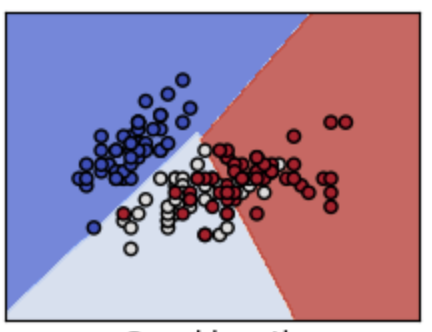
\includegraphics[scale=0.8]{imagenes/capitulo5/Entrenamiento/klineal.png}
	\caption{Kernel lineal}
	\label{fig:cp5:klineal}
	\end{subfigure}%
	\begin{subfigure}{.5\textwidth}
	\centering
	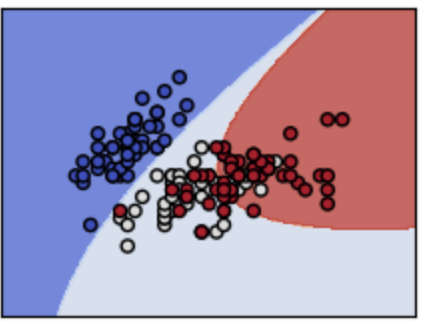
\includegraphics[scale=0.8]{imagenes/capitulo5/Entrenamiento/kpoli.png}
	\caption{Kernel polinomial}
	\label{fig:cp5:kpoli}
	\end{subfigure}%
\caption{Kernel de la función \citep{CC1}}
\end{figure}

\begin{figure}[H]
\centering
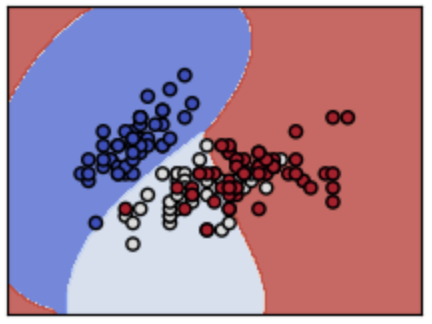
\includegraphics[scale=0.8]{imagenes/capitulo5/Entrenamiento/krbf.png}
\caption{Kernel radial \citep{CC1}}
\label{fig:cp5:krbf}
\end{figure}


Ahora se han explicado todos los parámetros de los algoritmos. Para las pruebas de este trabajo terminal han implementado 5 pliegues en la validación cruzada y se ha usado el corpus con 3150 noticias. Los resultados son visualizados en las siguientes tablas, donde la primera columna \textbf{Parámetros} contiene los parámetros variados de cada prueba, las columnas siguientes \textbf{P1}, \textbf{P2}, \textbf{P3}, \textbf{P4} y \textbf{P5} muestran el \textbf{exactitud} obtenido en cada pliegue, la columna \textbf{Promedio} muestra la suma de los \textbf{exactitud} obtenidos divido entre 5 (número de pliegues) y la última columna \textbf{Rank} muestra un número entero el cual indica el \textit{Ranking} de cada prueba, es decir la prueba con rank 1 es el mejor resultado, la prueba con rank 2 es el segundo mejor y así sucesivamente.\\

\begin{table}[H]
\centering
\resizebox{\columnwidth}{!}{%
	\begin{tabular}{|l|l|l|l|l|l|l|l|}
	%-----------------------Ecanbezado-----------------------------------%
		\hline
\multicolumn{1}{| >{\columncolor{myBlueChapter}}l|}{ \textcolor{myWhite}{\textbf{Parámetros}} }&
\multicolumn{1}{| >{\columncolor{myBlueChapter}}l|}{ \textcolor{myWhite}{\textbf{P 1}} }&
\multicolumn{1}{| >{\columncolor{myBlueChapter}}l|}{ \textcolor{myWhite}{\textbf{P 2}} }&
\multicolumn{1}{| >{\columncolor{myBlueChapter}}l|}{ \textcolor{myWhite}{\textbf{P 3}} }&
\multicolumn{1}{| >{\columncolor{myBlueChapter}}l|}{ \textcolor{myWhite}{\textbf{P 4}} }&
\multicolumn{1}{| >{\columncolor{myBlueChapter}}l|}{ \textcolor{myWhite}{\textbf{P 5}} }&
\multicolumn{1}{| >{\columncolor{myBlueChapter}}l|}{ \textcolor{myWhite}{\textbf{Promedio}} }&
\multicolumn{1}{| >{\columncolor{myBlueChapter}}l|}{ \textcolor{myWhite}{\textbf{Rank}} }
\\  \cline{1-8}
	%--------------

alpha: 0.5&0.8610&0.8576&0.8458&0.8487&0.8424&0.8511&1\\
\hline
alpha: 1&0.8531&0.8497&0.8426&0.8408&0.8360&0.8444&2\\
\hline
alpha: 1.5&0.8531&0.8434&0.8410&0.8392&0.8312&0.8416&3\\
\hline
alpha: 2&0.8531&0.8418&0.8410&0.8392&0.8296&0.8409&4\\
\hline

	\end{tabular}
}
\caption{Naive bayes}
\label{tab:cp5:naive}
\end{table}


\begin{table}[H]
\centering
\resizebox{\columnwidth}{!}{%
	\begin{tabular}{|l|l|l|l|l|l|l|l|}
	%-----------------------Ecanbezado-----------------------------------%
		\hline
\multicolumn{1}{| >{\columncolor{myBlueChapter}}l|}{ \textcolor{myWhite}{\textbf{Parámetros}} }&
\multicolumn{1}{| >{\columncolor{myBlueChapter}}l|}{ \textcolor{myWhite}{\textbf{P 1}} }&
\multicolumn{1}{| >{\columncolor{myBlueChapter}}l|}{ \textcolor{myWhite}{\textbf{P 2}} }&
\multicolumn{1}{| >{\columncolor{myBlueChapter}}l|}{ \textcolor{myWhite}{\textbf{P 3}} }&
\multicolumn{1}{| >{\columncolor{myBlueChapter}}l|}{ \textcolor{myWhite}{\textbf{P 4}} }&
\multicolumn{1}{| >{\columncolor{myBlueChapter}}l|}{ \textcolor{myWhite}{\textbf{P 5}} }&
\multicolumn{1}{| >{\columncolor{myBlueChapter}}l|}{ \textcolor{myWhite}{\textbf{Promedio}} }&
\multicolumn{1}{| >{\columncolor{myBlueChapter}}l|}{ \textcolor{myWhite}{\textbf{Rank}} }
\\  \cline{1-8}
	%--------------
C: 0.1, penalty: l2, solver: liblinear&0.8768&0.8655&0.8521&0.8710&0.8758&0.8682&1\\
\hline
C: 0.01, penalty: l2, solver: liblinear&0.8705&0.8655&0.8474&0.8742&0.8615&0.8638&2\\
\hline
C: 0.1, penalty: l1, solver: liblinear&0.8515&0.8544&0.8442&0.8424&0.8376&0.8460&3\\
\hline
C: 0.001, penalty: l2, solver: liblinear&0.8436&0.8560&0.8299&0.8392&0.8169&0.8371&4\\
\hline
C: 0.0001, penalty: l2, solver: liblinear&0.7836&0.7832&0.7806&0.7739&0.7723&0.7787&5\\
\hline
C: 0.01, penalty: l1, solver: liblinear&0.6477&0.6297&0.5946&0.6099&0.6099&0.6184&6\\
\hline
C: 1e-05, penalty: l2, solver: liblinear&0.6051&0.6044&0.6057&0.5924&0.5796&0.5974&7\\
\hline
C: 1e-06, penalty: l2, solver: liblinear&0.5261&0.5316&0.5564&0.5223&0.5048&0.5282&8\\
\hline
C: 1e-06, penalty: l1, solver: liblinear&0.2006&0.2009&0.2003&0.2006&0.2006&0.2006&9\\
\hline
C: 1e-05, penalty: l1, solver: liblinear&0.2006&0.2009&0.2003&0.2006&0.2006&0.2006&9\\
\hline
C: 0.0001, penalty: l1, solver: liblinear&0.2006&0.2009&0.2003&0.2006&0.2006&0.2006&9\\
\hline
C: 0.001, penalty: l1, solver: liblinear&0.2006&0.2009&0.2003&0.2006&0.2006&0.2006&9\\
\hline
	\end{tabular}
}
\caption{Regresión logística}
\label{tab:cp5:regresion}
\end{table}


\begin{table}[H]
\centering
\resizebox{\columnwidth}{!}{%
	\begin{tabular}{|l|l|l|l|l|l|l|l|}
	%-----------------------Ecanbezado-----------------------------------%
		\hline
\multicolumn{1}{| >{\columncolor{myBlueChapter}}l|}{ \textcolor{myWhite}{\textbf{Parámetros}} }&
\multicolumn{1}{| >{\columncolor{myBlueChapter}}l|}{ \textcolor{myWhite}{\textbf{P 1}} }&
\multicolumn{1}{| >{\columncolor{myBlueChapter}}l|}{ \textcolor{myWhite}{\textbf{P 2}} }&
\multicolumn{1}{| >{\columncolor{myBlueChapter}}l|}{ \textcolor{myWhite}{\textbf{P 3}} }&
\multicolumn{1}{| >{\columncolor{myBlueChapter}}l|}{ \textcolor{myWhite}{\textbf{P 4}} }&
\multicolumn{1}{| >{\columncolor{myBlueChapter}}l|}{ \textcolor{myWhite}{\textbf{P 5}} }&
\multicolumn{1}{| >{\columncolor{myBlueChapter}}l|}{ \textcolor{myWhite}{\textbf{Promedio}} }&
\multicolumn{1}{| >{\columncolor{myBlueChapter}}l|}{ \textcolor{myWhite}{\textbf{Rank}} }
\\  \cline{1-8}
	%--------------
max\_depth: 50, n\_estimators: 1000&0.8720&0.8592&0.8537&0.8631&0.8615&0.8619&1\\
\hline
max\_depth: 1000, n\_estimators: 1000&0.8689&0.8639&0.8585&0.8583&0.8583&0.8616&2\\
\hline
max\_depth: 100, n\_estimators: 1000&0.8752&0.8592&0.8569&0.8599&0.8551&0.8613&3\\
\hline
max\_depth: 100, n\_estimators: 500&0.8784&0.8608&0.8601&0.8535&0.8519&0.8609&4\\
\hline
max\_depth: 1000, n\_estimators: 500&0.8720&0.8528&0.8585&0.8551&0.8599&0.8597&5\\
\hline
max\_depth: 50, n\_estimators: 500&0.8705&0.8544&0.8601&0.8535&0.8599&0.8597&6\\
\hline
max\_depth: 500, n\_estimators: 1000&0.8720&0.8655&0.8506&0.8487&0.8583&0.8590&7\\
\hline
max\_depth: 500, n\_estimators: 500&0.8689&0.8544&0.8553&0.8519&0.8615&0.8584&8\\
\hline
max\_depth: 500, n\_estimators: 100&0.8610&0.8608&0.8506&0.8487&0.8662&0.8575&9\\
\hline
max\_depth: 50, n\_estimators: 100&0.8641&0.8528&0.8601&0.8503&0.8455&0.8546&10\\
\hline
max\_depth: 1000, n\_estimators: 100&0.8594&0.8528&0.8474&0.8392&0.8439&0.8485&11\\
\hline
max\_depth: 100, n\_estimators: 100&0.8657&0.8560&0.8394&0.8471&0.8280&0.8473&12\\
\hline
max\_depth: 50, n\_estimators: 50&0.8626&0.8402&0.8267&0.8583&0.8471&0.8470&13\\
\hline
max\_depth: 100, n\_estimators: 50&0.8420&0.8402&0.8283&0.8503&0.8535&0.8429&14\\
\hline
max\_depth: 500, n\_estimators: 50&0.8531&0.8418&0.8331&0.8424&0.8312&0.8403&15\\
\hline
max\_depth: 1000, n\_estimators: 50&0.8578&0.8212&0.8315&0.8392&0.8280&0.8355&16\\
\hline
	\end{tabular}
}
\caption{Random Forest}
\label{tab:cp5:random}
\end{table}


\begin{table}[H]
\centering
\resizebox{\columnwidth}{!}{%
	\begin{tabular}{|l|l|l|l|l|l|l|l|}
	%-----------------------Ecanbezado-----------------------------------%
		\hline
\multicolumn{1}{| >{\columncolor{myBlueChapter}}l|}{ \textcolor{myWhite}{\textbf{Parámetros}} }&
\multicolumn{1}{| >{\columncolor{myBlueChapter}}l|}{ \textcolor{myWhite}{\textbf{P 1}} }&
\multicolumn{1}{| >{\columncolor{myBlueChapter}}l|}{ \textcolor{myWhite}{\textbf{P 2}} }&
\multicolumn{1}{| >{\columncolor{myBlueChapter}}l|}{ \textcolor{myWhite}{\textbf{P 3}} }&
\multicolumn{1}{| >{\columncolor{myBlueChapter}}l|}{ \textcolor{myWhite}{\textbf{P 4}} }&
\multicolumn{1}{| >{\columncolor{myBlueChapter}}l|}{ \textcolor{myWhite}{\textbf{P 5}} }&
\multicolumn{1}{| >{\columncolor{myBlueChapter}}l|}{ \textcolor{myWhite}{\textbf{Promedio}} }&
\multicolumn{1}{| >{\columncolor{myBlueChapter}}l|}{ \textcolor{myWhite}{\textbf{Rank}} }
\\  \cline{1-8}
	%------------------------------------------------%
C: 100, gamma: 0.0001, kernel: rbf&0.8736&0.8639&0.8537&0.8726&0.8822&0.8692&1\\
\hline
C: 1000, gamma: 1e-05, kernel: rbf&0.8752&0.8623&0.8537&0.8710&0.8822&0.8689&2\\
\hline
C: 1000, gamma: 0.0001, kernel: rbf&0.8689&0.8608&0.8506&0.8694&0.8790&0.8657&3\\
\hline
C: 1, gamma: 0.0001, kernel: linear&0.8657&0.8592&0.8410&0.8710&0.8742&0.8622&4\\
\hline
C: 1, gamma: 1e-05, kernel: linear&0.8657&0.8592&0.8410&0.8710&0.8742&0.8622&4\\
\hline
C: 1, gamma: 1e-06, kernel: linear&0.8657&0.8592&0.8410&0.8710&0.8742&0.8622&4\\
\hline
C: 10, gamma: 0.0001, kernel: linear&0.8657&0.8592&0.8394&0.8710&0.8742&0.8619&5\\
\hline
C: 10, gamma: 1e-05, kernel: linear&0.8657&0.8592&0.8394&0.8710&0.8742&0.8619&5\\
\hline
C: 10, gamma: 1e-06, kernel: linear&0.8657&0.8592&0.8394&0.8710&0.8742&0.8619&5\\
\hline
C: 100, gamma: 0.0001, kernel: linear&0.8657&0.8592&0.8394&0.8710&0.8742&0.8619&5\\
\hline
C: 100, gamma: 1e-05, kernel: linear&0.8657&0.8592&0.8394&0.8710&0.8742&0.8619&5\\
\hline
C: 100, gamma: 1e-06, kernel: linear&0.8657&0.8592&0.8394&0.8710&0.8742&0.8619&5\\
\hline
C: 1000, gamma: 0.0001, kernel: linear&0.8657&0.8592&0.8394&0.8710&0.8742&0.8619&5\\
\hline
C: 1000, gamma: 1e-05, kernel: linear&0.8657&0.8592&0.8394&0.8710&0.8742&0.8619&5\\
\hline
C: 1000, gamma: 1e-06, kernel: linear&0.8657&0.8592&0.8394&0.8710&0.8742&0.8619&5\\
\hline
C: 10, gamma: 0.0001, kernel: rbf&0.8641&0.8576&0.8490&0.8678&0.8503&0.8578&6\\
\hline
C: 100, gamma: 1e-05, kernel: rbf&0.8641&0.8576&0.8490&0.8662&0.8519&0.8578&6\\
\hline
C: 1000, gamma: 1e-06, kernel: rbf&0.8641&0.8576&0.8490&0.8662&0.8519&0.8578&6\\
\hline
C: 100, gamma: 1e-06, kernel: rbf&0.6524&0.6772&0.6073&0.6449&0.6608&0.6485&7\\
\hline
C: 10, gamma: 1e-05, kernel: rbf&0.6493&0.6741&0.6073&0.6401&0.6561&0.6454&8\\
\hline
C: 1, gamma: 0.0001, kernel: rbf&0.6193&0.6440&0.5946&0.6115&0.6306&0.6200&9\\
\hline
C: 1, gamma: 0.0001, kernel: poly&0.2038&0.2041&0.2035&0.2038&0.2038&0.2038&10\\
\hline
C: 1, gamma: 1e-05, kernel: poly&0.2038&0.2041&0.2035&0.2038&0.2038&0.2038&10\\
\hline
C: 1, gamma: 1e-05, kernel: rbf&0.2038&0.2041&0.2035&0.2038&0.2038&0.2038&10\\
\hline
C: 1, gamma: 1e-06, kernel: poly&0.2038&0.2041&0.2035&0.2038&0.2038&0.2038&10\\
\hline
C: 1, gamma: 1e-06, kernel: rbf&0.2038&0.2041&0.2035&0.2038&0.2038&0.2038&10\\
\hline
C: 10, gamma: 0.0001, kernel: poly&0.2038&0.2041&0.2035&0.2038&0.2038&0.2038&10\\
\hline
C: 10, gamma: 1e-05, kernel: poly&0.2038&0.2041&0.2035&0.2038&0.2038&0.2038&10\\
\hline
C: 10, gamma: 1e-06, kernel: poly&0.2038&0.2041&0.2035&0.2038&0.2038&0.2038&10\\
\hline
C: 10, gamma: 1e-06, kernel: rbf&0.2038&0.2041&0.2035&0.2038&0.2038&0.2038&10\\
\hline
C: 100, gamma: 0.0001, kernel: poly&0.2038&0.2041&0.2035&0.2038&0.2038&0.2038&10\\
\hline
C: 100, gamma: 1e-05, kernel: poly&0.2038&0.2041&0.2035&0.2038&0.2038&0.2038&10\\
\hline
C: 100, gamma: 1e-06, kernel: poly&0.2038&0.2041&0.2035&0.2038&0.2038&0.2038&10\\
\hline
C: 1000, gamma: 0.0001, kernel: poly&0.2038&0.2041&0.2035&0.2038&0.2038&0.2038&10\\
\hline
C: 1000, gamma: 1e-05, kernel: poly&0.2038&0.2041&0.2035&0.2038&0.2038&0.2038&10\\
\hline
C: 1000, gamma: 1e-06, kernel: poly&0.2038&0.2041&0.2035&0.2038&0.2038&0.2038&10\\
\hline

	\end{tabular}
}
\caption{Máquina de soporte vectorial}
\label{tab:cp5:msv}
\end{table}




%------------------------------------------------------------------%
\subsection{Selección}


Los resultados de la sección anterior ha mostrado que no existe una brecha muy grande en el \textbf{exactitud} obtenido de los mejores parámetros, como se muestra en la siguiente Tabla (\ref{tab:cp5:resultados}).

\begin{table}[H]
\centering
	\begin{tabular}{|l|c|c|}
	%-----------------------Ecanbezado-----------------------------------%
		\hline
\multicolumn{1}{| >{\columncolor{myBlueChapter}}l|}{ \textcolor{myWhite}{\textbf{Algoritmo}} }&
\multicolumn{1}{| >{\columncolor{myBlueChapter}}l|}{ \textcolor{myWhite}{\textbf{Exactitud}} }&
\multicolumn{1}{| >{\columncolor{myBlueChapter}}l|}{ \textcolor{myWhite}{\textbf{Ranking}} }
\\  \cline{1-3}
	%--------------

MSV&0.8692&1\\
\hline
Regresión Logística&0.8682&2\\
\hline
Random Forest&0.8619&3\\
\hline
Naive Bayes&0.8511&4\\
\hline
	\end{tabular}
\caption{Precisión de los mejores parámetros}
\label{tab:cp5:resultados}
\end{table}


El mejor resultado se ha conseguido con el algoritmo \textbf{Máquina de soporte vectorial} con los parámetros ;$C$=100, $gamma$=0.0001 y $kernel$= $rbf$ (radial) obteniendo 0.8619 de \textbf{exactitud}, por esta razón se ha elegido como el clasificador final de este trabajo terminal.

%------------------------------------------------------------------%
\subsection{Pruebas}

Con base en el algoritmo elegido y los parámetros que han conseguido obtener el mejor resultado, se ha hecho una prueba final, la cual consiste en clasificar el corpus de prueba con 350 noticias, creado al final de la sección de pre-procesamiento (ver \Tref{cp5:divisionC}{División del corpus}  ), para calcular la matriz de confusión y obtener las métricas de evaluación. La tabla \ref{tab:cp5:numnoticias} muestra el número de noticias por sección contenidas en el corpus.\\

\begin{table}[H]
\centering
	\begin{tabular}{|l|c|}
	%-----------------------Ecanbezado-----------------------------------%
		\hline
\multicolumn{1}{| >{\columncolor{myBlueChapter}}l|}{ \textcolor{myWhite}{\textbf{Sección}} }&
\multicolumn{1}{| >{\columncolor{myBlueChapter}}l|}{ \textcolor{myWhite}{\textbf{Número de noticias}} }
\\  \cline{1-2}
	%--------------

Deportes& 68\\
\hline
Economía& 58\\
\hline
Política& 69\\
\hline
Cultura& 77\\
\hline
Ciencia y Tecnología& 78\\
\hline
	\end{tabular}
\caption{Número de noticias}
\label{tab:cp5:numnoticias}
\end{table}


La matriz de confusión obtenida se muestra en la tabla \ref{tab:cp5:matriz}, donde las filas representan la clasificación real de la noticia y las columnas lo predicho por el clasificador. Por ejemplo se observa que en la sección \textbf{Deportes} de 68 noticias etiquetadas, 65 fueron clasificadas correctamente, y 3 fueron mal clasificadas en la sección \textbf{ciencia y tecnología} (1 noticia), \textbf{economía} (1 noticia) y \textbf{política} (1 noticia). En la sección de ciencia y tecnología de 78 noticias solo 67 fueron clasificadas de forma acertada, y 11 fueron clasificadas en las distintas secciones: 1 en \textbf{Deportes}, 5 en \textbf{Economía}, 3 en \textbf{Política} y 2 en \textbf{Cultura}.\\

\begin{table}[H]
\centering
\resizebox{\columnwidth}{!}{%
	\begin{tabular}{|l|c|c|c|c|c|}
	%-----------------------Ecanbezado-----------------------------------%
		\hline
\multicolumn{1}{| >{\columncolor{myBlueChapter}}l|}{ \textcolor{myWhite}{\textbf{Sección}} }&
\multicolumn{1}{| >{\columncolor{myBlueChapter}}l|}{ \textcolor{myWhite}{\textbf{Deportes}} }&
\multicolumn{1}{| >{\columncolor{myBlueChapter}}l|}{ \textcolor{myWhite}{\textbf{Economía}} }&
\multicolumn{1}{| >{\columncolor{myBlueChapter}}l|}{ \textcolor{myWhite}{\textbf{Política}} }&
\multicolumn{1}{| >{\columncolor{myBlueChapter}}l|}{ \textcolor{myWhite}{\textbf{Cultura}} }&
\multicolumn{1}{| >{\columncolor{myBlueChapter}}l|}{ \textcolor{myWhite}{\textbf{Cienci y T}} }
\\  \cline{1-6}
	%--------------

Deportes& 65 & 1 & 1 & 0 & 1\\
\hline
Economía& 1 & 51 & 4 & 1 & 1\\
\hline
Política& 2 & 5 & 59 & 3 & 0\\
\hline
Cultura& 1 & 1 & 1 & 70 & 4\\
\hline
Ciencia y T& 1 & 5 & 3 & 2 & 67\\
\hline
	\end{tabular}
}
\caption{Matriz de confusión}
\label{tab:cp5:matriz}
\end{table}


Con base en la matriz de confusión se ha calculado \textbf{Recall}, \textbf{Fmeasure}, \textbf{Precision} (ver \Tref{cp3:metricase}{Métricas de evaluación}). Las métricas son obtenidas por cada sección, como se muestra en la tabla \ref{tab:cp5:metricas}.

\begin{table}[H]
\centering
	\begin{tabular}{|l|c|c|c|}
	%-----------------------Ecanbezado-----------------------------------%
		\hline
\multicolumn{1}{| >{\columncolor{myBlueChapter}}l|}{ \textcolor{myWhite}{\textbf{Sección}} }&
\multicolumn{1}{| >{\columncolor{myBlueChapter}}l|}{ \textcolor{myWhite}{\textbf{Precision}} }&
\multicolumn{1}{| >{\columncolor{myBlueChapter}}l|}{ \textcolor{myWhite}{\textbf{Recall}} }&
\multicolumn{1}{| >{\columncolor{myBlueChapter}}l|}{ \textcolor{myWhite}{\textbf{F-measuere}} }
\\  \cline{1-4}
	%--------------

Deportes & 0.93 & 0.96 & 0.94\\
\hline
Economía & 0.81 & 0.88 & 0.84\\
\hline
Política & 0.87 & 0.86 & 0.86\\
\hline
Cultura & 0.92 & 0.91 & 0.92\\
\hline
Ciencia y Tecnología & 0.92 & 0.86 & 0.89\\
\hline
	\end{tabular}
\caption{Metricas de evaluación}
\label{tab:cp5:metricas}
\end{table}


Como se puede observar en la tabla \ref{tab:cp5:metricas} las sección con mejor \textbf{Fmeasure} (este valor sostiene una relación entre \textbf{Precision} y \textbf{Recall}) es \textbf{Deportes} obteniendo 0.94 en la clasificación. Este resultado se puede explicar con base en el vocabulario manejado en la categoría, ya que es muy específico, por ejemplo se usan palabras como: gol, jugador, resultado, anotación. Por lo contrario el \textbf{Fmeasure} mas bajo lo obtuvo \textbf{Economía} con 0.84 (el cual no es un mal resultado), las palabras manejadas por esta sección pueden ser encontradas en otras categorías, generando así confusión en la clasificación.\\

Finalmente, considerando la exactitud de de todas las secciones, el modelo entrenado obtuvo una exactitud promedio de 0.89. Este resultado es muy bueno considerando que los trabajos descritos en el estado del arte (ver \Tref{cp2:estadodelarte}{Estado del arte}) obtienen una exactitud entre 0.80 y 0.90




%------------------------------------------------------------------%
\Tlabel{cp5:persistencia}
\subsection{Persistencia}


Como última etapa de la clasificación, el modelo \textbf{Máquina de soporte vectorial} debe ser almacenado así como las características del corpus. Para esta tarea se ha utilizado el corpus completo de 3500 noticias, del cual se extraen las características, se entrena el modelo y estos conjuntos son almacenados en un archivo ocupando la biblioteca \textbf{pickle}, de esta forma en la siguiente sección el modelo es utilizado como parte de la \textbf{Aplicación web}.



%\subsection{Tokenizar}
%\subsection{Lematizar}
%\subsection{Validación cruzada}
%\subsection{Shuffle}
%\subsection{Grid search}
%\subsection[Resultados]{Selección y resultado del mejor clasificador}
%\subsection[Persistencia]{Persistencia del clasificador}
\newpage
\section{Aplicación web}

La siguiente Figura \ref{fig:procesoApp} muestra las etapas que se llevarán a cabo por parte de la aplicación web.
\begin{figure}[ht]
\centering
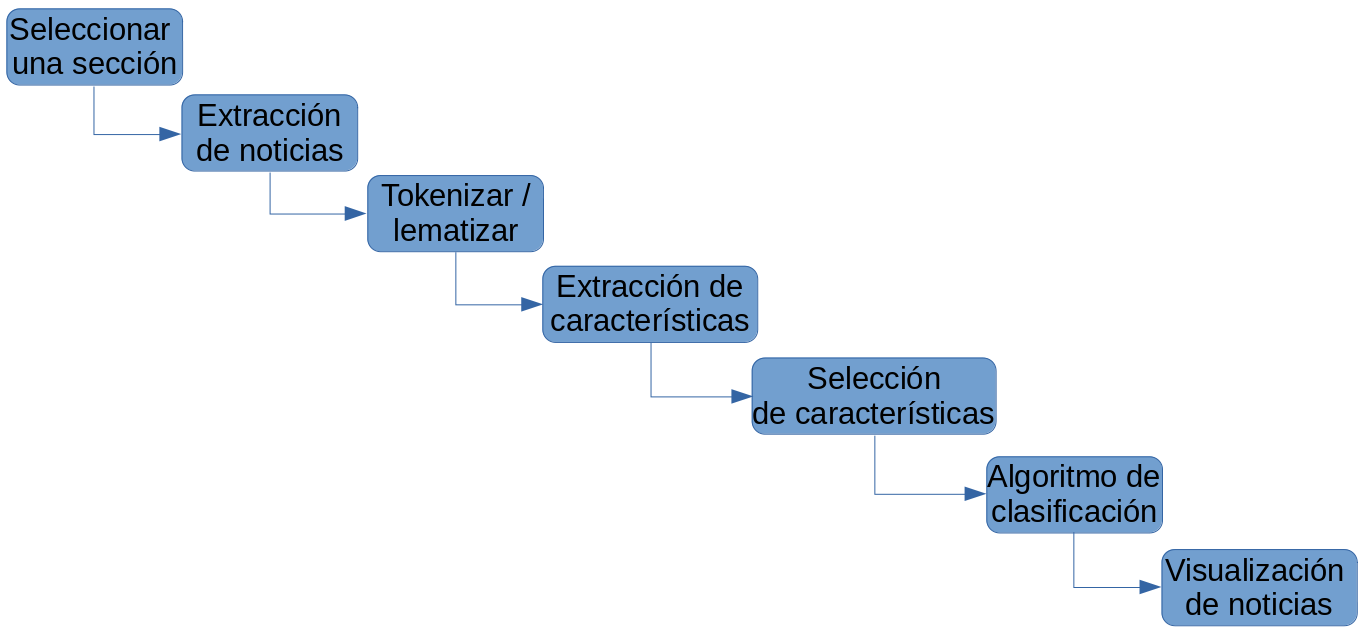
\includegraphics[scale=0.3]{imagenes/Capitulo5/procesoAplicacionWeb.png}
\caption{Etapas de la aplicación web}
\label{fig:procesoApp}
\end{figure}

\subsection{Proceso de recolección}
La aplicación web tiene como objetivo recolectar y clasificar noticias, por ello la primera parte que se debe realizar es la recolección de noticias, como se mencionó en el apartado 5.1 se han definido los sitios web de donde las noticias serán recolectadas, la información recuperada śerá:

\begin{itemize}
	\item URL de la noticia
	\item Título
	\item Fecha
	\item Autor
	\item Descripción \footnote{Existen sitios web, donde no todas las noticias cuentan con una descripción}
	\item Noticia
\end{itemize}

Cabe destacar que en este punto, ya no será necesario extraer el nombre de la sección a la cual pertenece la noticia.
\\
\subsection{Proceso de clasificación}
Una vez que las noticias han sido recolectadas, deberán pasar por dos pasos fundamentales, como primer paso la noticia debe ser tokenizada y lematizada, posteriormente se deben extraer las características de cada noticia, esto permitirá al algoritmo seleccionado tener una mejor precisión en el momento de realizar la clasificación, 
para finalizar las noticias serán clasificadas.

\subsection{Frontend}

Para la realización de la aplicación web es necesario utilizar herramientas que nos permitan visualizar las noticias clasificadas, por ello las interfaces de usuario se desarrollarón en utilizando el Framework Java Server Faces.

La Figura \ref{fig:PantallaInicio} muestra la vista que tendrá el usuario al ingresar a la aplicación web

\begin{figure}[ht]
\centering
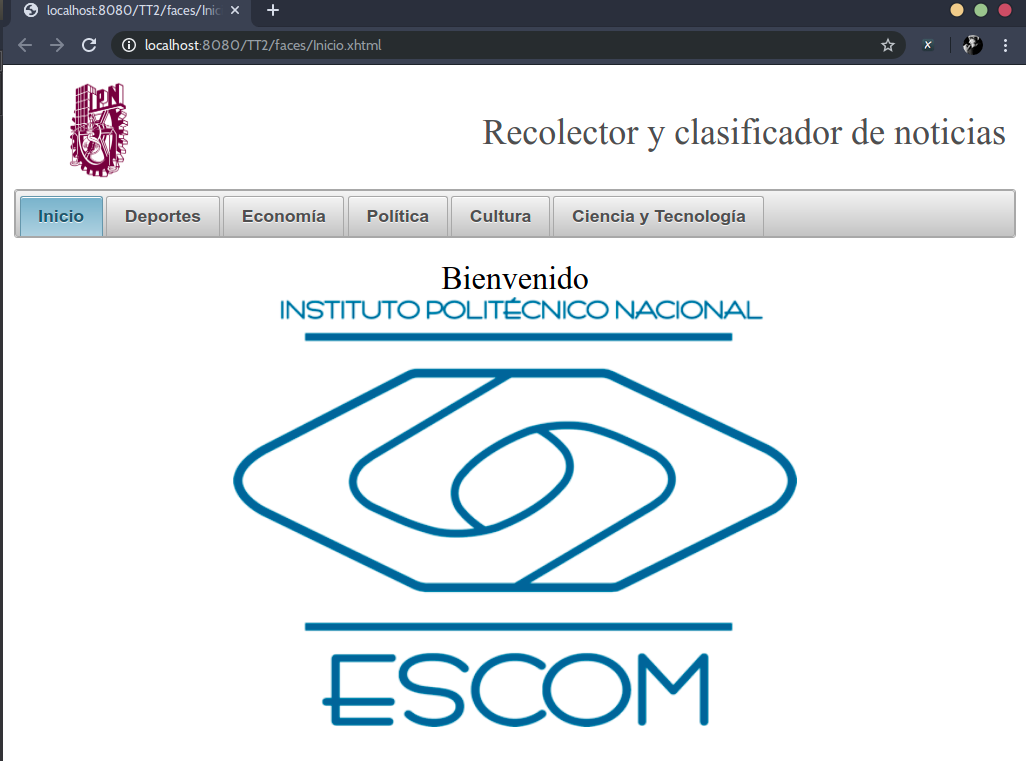
\includegraphics[scale=0.3]{imagenes/Capitulo5/inicio.png}
\caption{Pantalla de Inicio.}
\label{fig:PantallaInicio}
\end{figure}

El usuario tiene la posibilidad de elegir la sección de la cual desee visualizar noticias. La Figura \ref{fig:loading} muestra la vista que tendrá el usuario dar click en una sección.

\begin{figure}[ht]
\centering
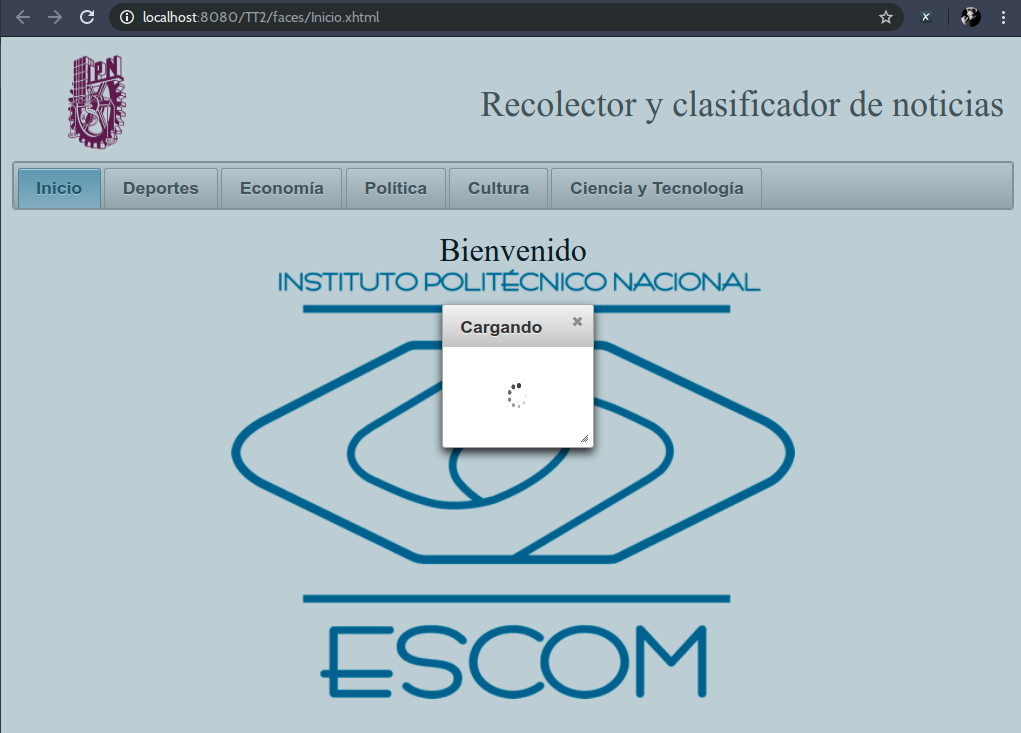
\includegraphics[scale=0.3]{imagenes/Capitulo5/cargando.png}
\caption{Pantalla de espera}
\label{fig:loading}
\end{figure}

Una vez finalizado el proceso de recolección de noticias


El proceso que se llevará a cabo para poder visualizar 
Para visualizar
	Aplicación web
		Archivo físico
		ya no se busca por sección 
		hacer menció de casos de uso

\newpage


